\chapter{UAV sensing 3D phenotyping pipeline for harvestable organs}

% This section has been modified and submitted to the ``Plant Phenomics"

\begin{center}
  \noindent
  \fbox{
    \begin{minipage}{0.95\textwidth}
    
      \begin{center}
        \textbf{Drone-based harvest data prediction can reduce on-farm food loss and improve farmer income}
      \end{center}

      \noindent Haozhou Wang$^{1}$, Tang Li$^{1}$, Erika Nishida$^{1}$, Yoichiro Kato$^{1}$, Yuya Fukano$^{2\star}$, and Wei Guo$^{1,\star}$
    
      \noindent $^{1}$ Graduate School of Agricultural and Life Sciences, The University of Tokyo, Tokyo, Japan
      
      \noindent $^{2}$ Graduate School of Horticulture, Chiba University, Chiba, Japan
      
      \noindent $^{\star}$ Corresponding authors

      \begin{spacing}{1.5}
      \textbf{Abstract}
      \end{spacing}
      
      On-farm food loss (i.e., grade-out vegetables) is a difficult challenge in sustainable agricultural systems. The simplest method to reduce the number of grade-out vegetables is to monitor and predict the size of all individuals in the vegetable field and determine the optimal harvest date. Here, we developed a full pipeline to accurately estimate and predict every broccoli head size (n $>$ 3000) automatically and nondestructively using drone remote sensing and image analysis and predicted the optimal harvesting date. Two years of field experiments revealed that our pipeline successfully estimated and predicted the head size of all broccolis with high accuracy. We successfully predicted the optimal harvest date and found that a deviation of only 1‒2 d from that date can significantly increase grade-out and reduce farmer profits. This is an unequivocal demonstration of the utility of these approaches to economic crop optimization and minimization of food losses. A short video that summarized this study can be found here: \url{https://youtu.be/SYuOCVqgtrU}

      \vspace{5mm}
      \textbf{keywords}: unmanned aerial vehicle (UAV), time-series analysis, deep learning, YOLO, BiSeNet

    \end{minipage}
  }
\end{center}

\section{Introduction}

Waste caused by non-standard vegetables is an unavoidable component of food loss in modern society \citep{parfitt_food_2010,teuber_food_2016}. The vegetables do not meet the cosmetic standards (e.g. size, shape, and aesthetics) cannot be easily sold and are not harvested \citep{garrone_opening_2014}. \citet{porter_avoidable_2018} estimated that over one-third of the total agricultural production (e.g., 51,500 kilotons annually in the European Economic Area) is lost for this reason. Furthermore, owing to the uneven growth rate of individual vegetables and one-time mechanical reaping, some vegetables are not harvested at the appropriate time and thus are discarded. Although the conventional method of selective harvesting by hand several times during the growing season could minimize such waste, the labor cost (107 person-hours per hectare) eliminates its profits \citep{blok_effect_2021}. Thus, the development of technologies to monitor and measure the status of each harvestable organ of the whole field is of great value.

% Waste caused by non-standard vegetables is an unavoidable component of food loss in modern society \citep{parfitt_food_2010,teuber_food_2016}. Cosmetic standards (e.g., size, shape, and aesthetics) play an important role in vegetable quality standards in Northern Hemisphere countries \citep{porter_avoidable_2018}. Therefore, vegetables that do not meet this standard cannot be easily sold and are not harvested \citep{garrone_opening_2014}. \citet{porter_avoidable_2018} estimated that over one-third of the total agricultural production (e.g., 51,500 kilotons annually in the European Economic Area) is lost for this reason. For vegetables harvested by mechanical reaping, owing to the uneven growth rate of individual vegetables, some are not harvested at the appropriate time and are discarded. Hence, the development of technologies to predict the optimal time for the whole field harvesting not only increases the effective yield and profit of farmers, but also contributes to sustainable development and the global environment (Sustainable Development Goals [SDG] targets 12.3 and 12.5).

% Broccoli (\textit{Brassica oleracea} L.) head is an important component of the global vegetable market; however, there is a high percentage of on-farm waste. Its non-edible parts (leaves, stems) account for $> 75\%$ of the above-ground biomass \citep[Table~1]{fink_nitrogen_1999}. For the remaining marketable parts, the variable bud growth rate results in large variations in head size under complex field conditions. As for other vegetables, fresh broccoli has shipping standards (head diameter, weight, shape, etc.); therefore, a certain amount of non-standard harvested head is wasted from one-time mechanical harvesting. Although the conventional method of selective harvesting by hand three times during the growing season could minimize such waste, the labor cost (107 person-hours per hectare) eliminates its profits \citep{blok_effect_2021}. Because the shipping price is highly dependent on head size, the harvest date is essential to determine the proportion of non-standard-size broccoli and the total income for farmers. If the size distribution of all individuals in the broccoli field could be determined and predicted in the short term, it would be possible to set the optimal harvest date to reduce the number of non-standard-size vegetables and minimize food losses. However, it is unrealistic to manually determine the size distribution of all broccoli in the field.

Smart farming, which involves new technologies such as remote sensing, high-throughput phenotyping, and artificial intelligence in agricultural production, has received considerable attention from researchers, farmers, and governments. The UAV-based pipeline provides a flexible and cost-efficient method to capture images for vegetable canopies. The 3D canopy model can also be reconstructed using photogrammetry-based software. Several studies extended this approach to estimate the canopy architectural traits \citep{shu_application_2021, wang_detection_2021, herrero_canopy_2020} and even traits for individual lettuce \citep{bauer_combining_2019}. But such canopy-level or individual-level can not meet the accuracy demand for harvestable organ size judgment; for example, the broccoli head grades vary by a few centimeters. Therefore, extracting the organ-level traits can significantly improve the accuracy of whole-field estimation.

For many organ-level applications, the images are often collected close to the ground by a hand-held camera or an unmanned ground vehicle (UGV). Although several studies successfully proved the accuracy and feasibility of this approach on small-area experimental fields \citep{luling_using_2021,garcia_towards_2021,blok_effect_2021}, its efficiency is not always applicable to the large-area field with thousands of crops, compared to the UAV-based approach. To apply the organ-level analysis on the UAV-based approach, there are two main challenges to be solved.

One challenge is the poor quality of the reconstructed canopy model (2D field map and 3D point cloud). Due to the plant structure movement in different UAV images caused by wind, the canopy model often has the effects of double mapping (ghost effect) and seamline distortion \citep{lin_new_2021}; as the Figure~\ref{fig:idp1}b shows. Many studies tried to fix the low quality using machine learning algorithms \citep{hu_pixel_2019,hu_coupling_2021,velumani_estimates_2021} or multi-spectral sensors \citep{guo_wheat_2021,lu_assessment_2022}, these can be time-consuming, costly, and are often not robust on different crops. Little attention has been paid to the original UAV images which often have better quality, due to the drawback of directly analyzing the images is unable to identify the results to which crop in the field without detailed GPS locations like the canopy model. One solution is to reuse the geometric relationship between UAV images and the field model generated by 3D reconstruction (Fig.~\ref{fig:idp1}c). \citet{duan_comparison_2017,guo_aerial_2018} tested this idea to find the canopy-level corresponding place on original UAV images from the Pix4D reconstructed canopy model, while \citet{lin_new_2021} developed their own algorithms to fix the field map. But they did not publish any source code or tools, making it unreachable to agricultural users who do not have solid photogrammetry backgrounds and professional programming skills.

\begin{figure}[htb]
  \begin{center}
    \resizebox{\textwidth}{!}{
      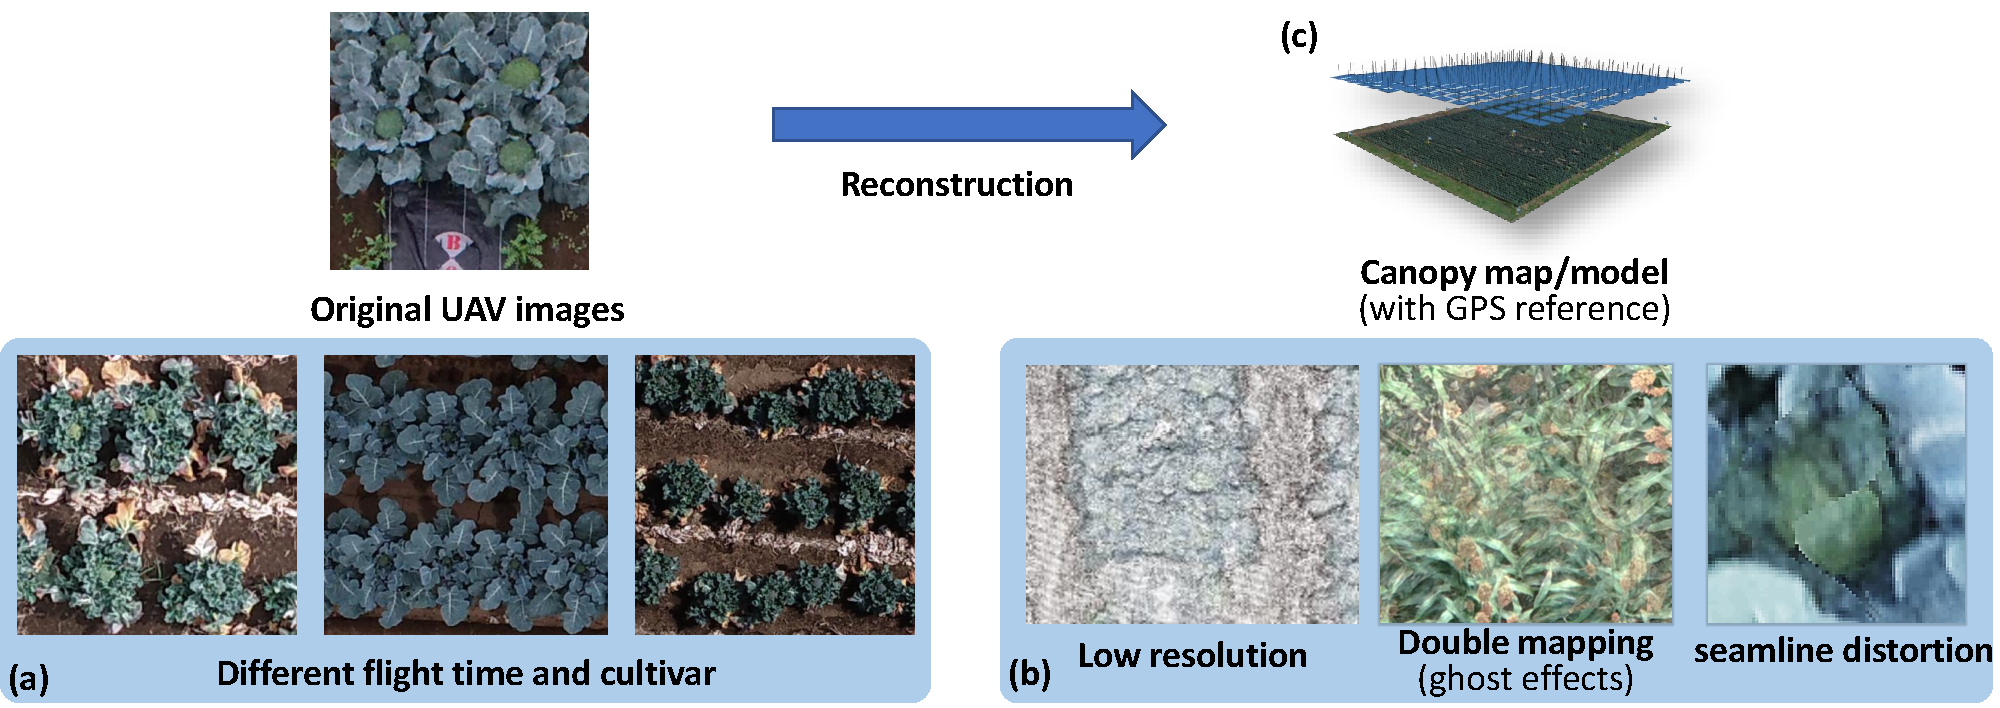
\includegraphics{figures/idp/Fig.1_background.pdf}
    }
  \end{center}
  \caption[Organ-level analysis challenges of UAV-based approach]{
    The main challenges for organ-level analysis on the UAV-based approach. (a) shows the produced canopy 2D map and 3D model often have poor qualify, and suffer from double mapping (ghost effect) and seamline distortion. (b) shows the huge differences time, sunlight, soil condition, growing stage, and cultivars, which makes the image analysis is quite difficult. (c) is a figure to show the relationship between raw UAV images and the reconstructed canopy model.
  }
  \label{fig:idp1}
\end{figure}

The other challenge is the complexity of crop images. As Figure~\ref{fig:idp1}a shows, there are huge differences between time, sunlight, soil condition, growing stage, and cultivar. It is quite difficult to design a conventional computer vision algorithm to handle all of them at the same time. Many studies have applied deep learning algorithms on the broccoli head image segmentation tasks \citep{garcia_towards_2021,blok_image_2021,zhou_monitoring_2020}, but most of them took images under controlled conditions (indoor or inside a black box). To fulfill the more complex outdoor tasks, a large amount of training data need to be manually labeled. Though there is a public training dataset for growliflower available \citep{kierdorf_growliflower_2022}, it can not be used directly on the broccoli head or another crop. Besides, labeling 14,000 individual crops manually like that dataset is not feasible for all kinds of crops. To decrease the workload of this deep learning solution, it is preferable to simplify the image segmentation, minimize the number of computation tasks, and increase the efficiency of training data acquisition as much as possible.

% Smart farming, which involves new technologies such as machinery, remote sensing, high-throughput phenotyping, and artificial intelligence in agricultural production, has received considerable attention from researchers, farmers, and governments. The unmanned aerial vehicle (UAV)-based pipeline provides a flexible and cost-efficient method to capture high-resolution images using various lightweight sensors. By using high-resolution UAV images captured over time, it may be possible to estimate the growth of the head size of all individual vegetables. The time-series data of the head size distribution of all broccoli can be used to develop a prediction model for the short-term growth of broccoli heads. If the head size of all individuals can be predicted, combined with the market prices for each size grade, a prediction system for the optimal harvest date can be built. 

% However, several challenges must be overcome to develop a broccoli head size estimation pipeline. First, broccoli grades vary by a few centimeters; therefore, a highly accurate estimation is required. In particular, for UAV images from the broccoli field, the head can be hidden by leaves. Second, for agricultural field applications, it is preferable to minimize the number of computation tasks as much as possible. In particular, semantic segmentation for each crop or organ was obtained from images of the entire field using deep learning \citep{bauer_combining_2019,zhou_automated_2022}. Third, deep learning model training is often powered by a large amount of training data and annotations. Efficient acquisition of these data is an urgent need for deep learning applications in agriculture \citep{kierdorf_growliflower_2022}.

In this study, we developed several techniques (backward projection, pre-position-guided head segmentation, and interactive annotation) to overcome the aforementioned challenges and provide a highly accurate and labor-saving pipeline for broccoli head size estimation. The goals of this study were to: (1) develop a general workflow of the broccoli head size estimation pipeline; (2) implement the pipeline for field trials of broccoli growth in 2020 and 2021; and (3) validate the estimated head size by comparison with field measurements. This pipeline also has great potential to be seamlessly interfaced with other cabbage-like crops, including cauliflower, artichoke, and even lettuce. Meanwhile, the use of a simple RGB sensor, not a complex integration of multiple or expensive sensors (i.e., multi-spectral, LiDAR), makes it more applicability and user-friendly for the farmers, farming and the economic sustainability of many economically and socially disadvantaged rural regions. 

\section{Methods}

The general workflow of the broccoli head size measurement pipeline is shown in Fig.~\ref{fig:bro4} and the Supplementary Video \ref{spp:video}. The time-series data of all broccoli were collected and visualized using a UAV-based pipeline. The pipeline included the following steps:1) aerial data collection; 2) data preprocessing and 3D reconstruction; 3) broccoli position detection using YOLO v5 at the seedling stage; 4) broccoli head segmentation using BiSeNet v2, and; 5) geometry trait calculation. 

% Second, a simple growth model was built using the head size and temperature data. Finally, a profit prediction model was generated according to the market price survey.

\begin{figure}[htb]
  \begin{center}
    \resizebox{0.6\textwidth}{!}{
      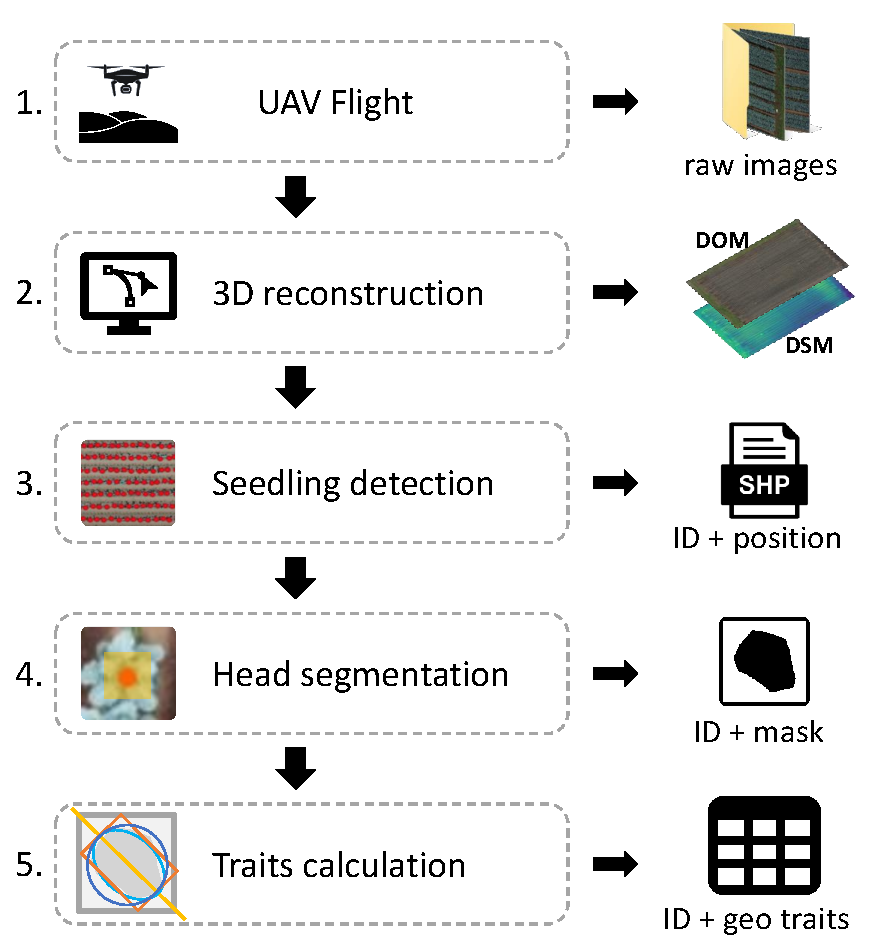
\includegraphics{figures/bro/Fig.4_general_workflow.pdf}
    }
  \end{center}
  \caption[Workflow and schematic of the UAV-based pipeline]{
    Workflow and schematic of the UAV-based pipeline which was used to obtain the time-series head size information (geometry traits) of all broccoli heads during the growing season (the outputs of each step are the inputs of the next step).
  }
  \label{fig:bro4}
\end{figure}

\subsection{Plot conditions and field data collection}

Field trials were conducted at the experimental farm of the Institute for Sustainable Agro-ecosystem Services (ISAS), Nishi-Tokyo, Tokyo, Japan ($35^\circ 43'$N, $139^\circ 32'$E) in 2020 and 2021 (Fig.~\ref{fig:bro5}). Detailed meteorological data during the growth period were collected by a local weather station and are shown in Supplementary Table ~\ref{fig:bros2}. The plot sizes were approximately 0.2 and 0.1 ha for 2020 and 2021, respectively. During the 2-year experiment, the same broccoli cultivar (Jet dome) was planted under the same field management. Machine planting of seedlings at 35-cm intervals in rows 70 cm apart is consistent with local commercial broccoli cultivation regimes. 

\begin{figure}[htb]
  \begin{center}
    \resizebox{\textwidth}{!}{
      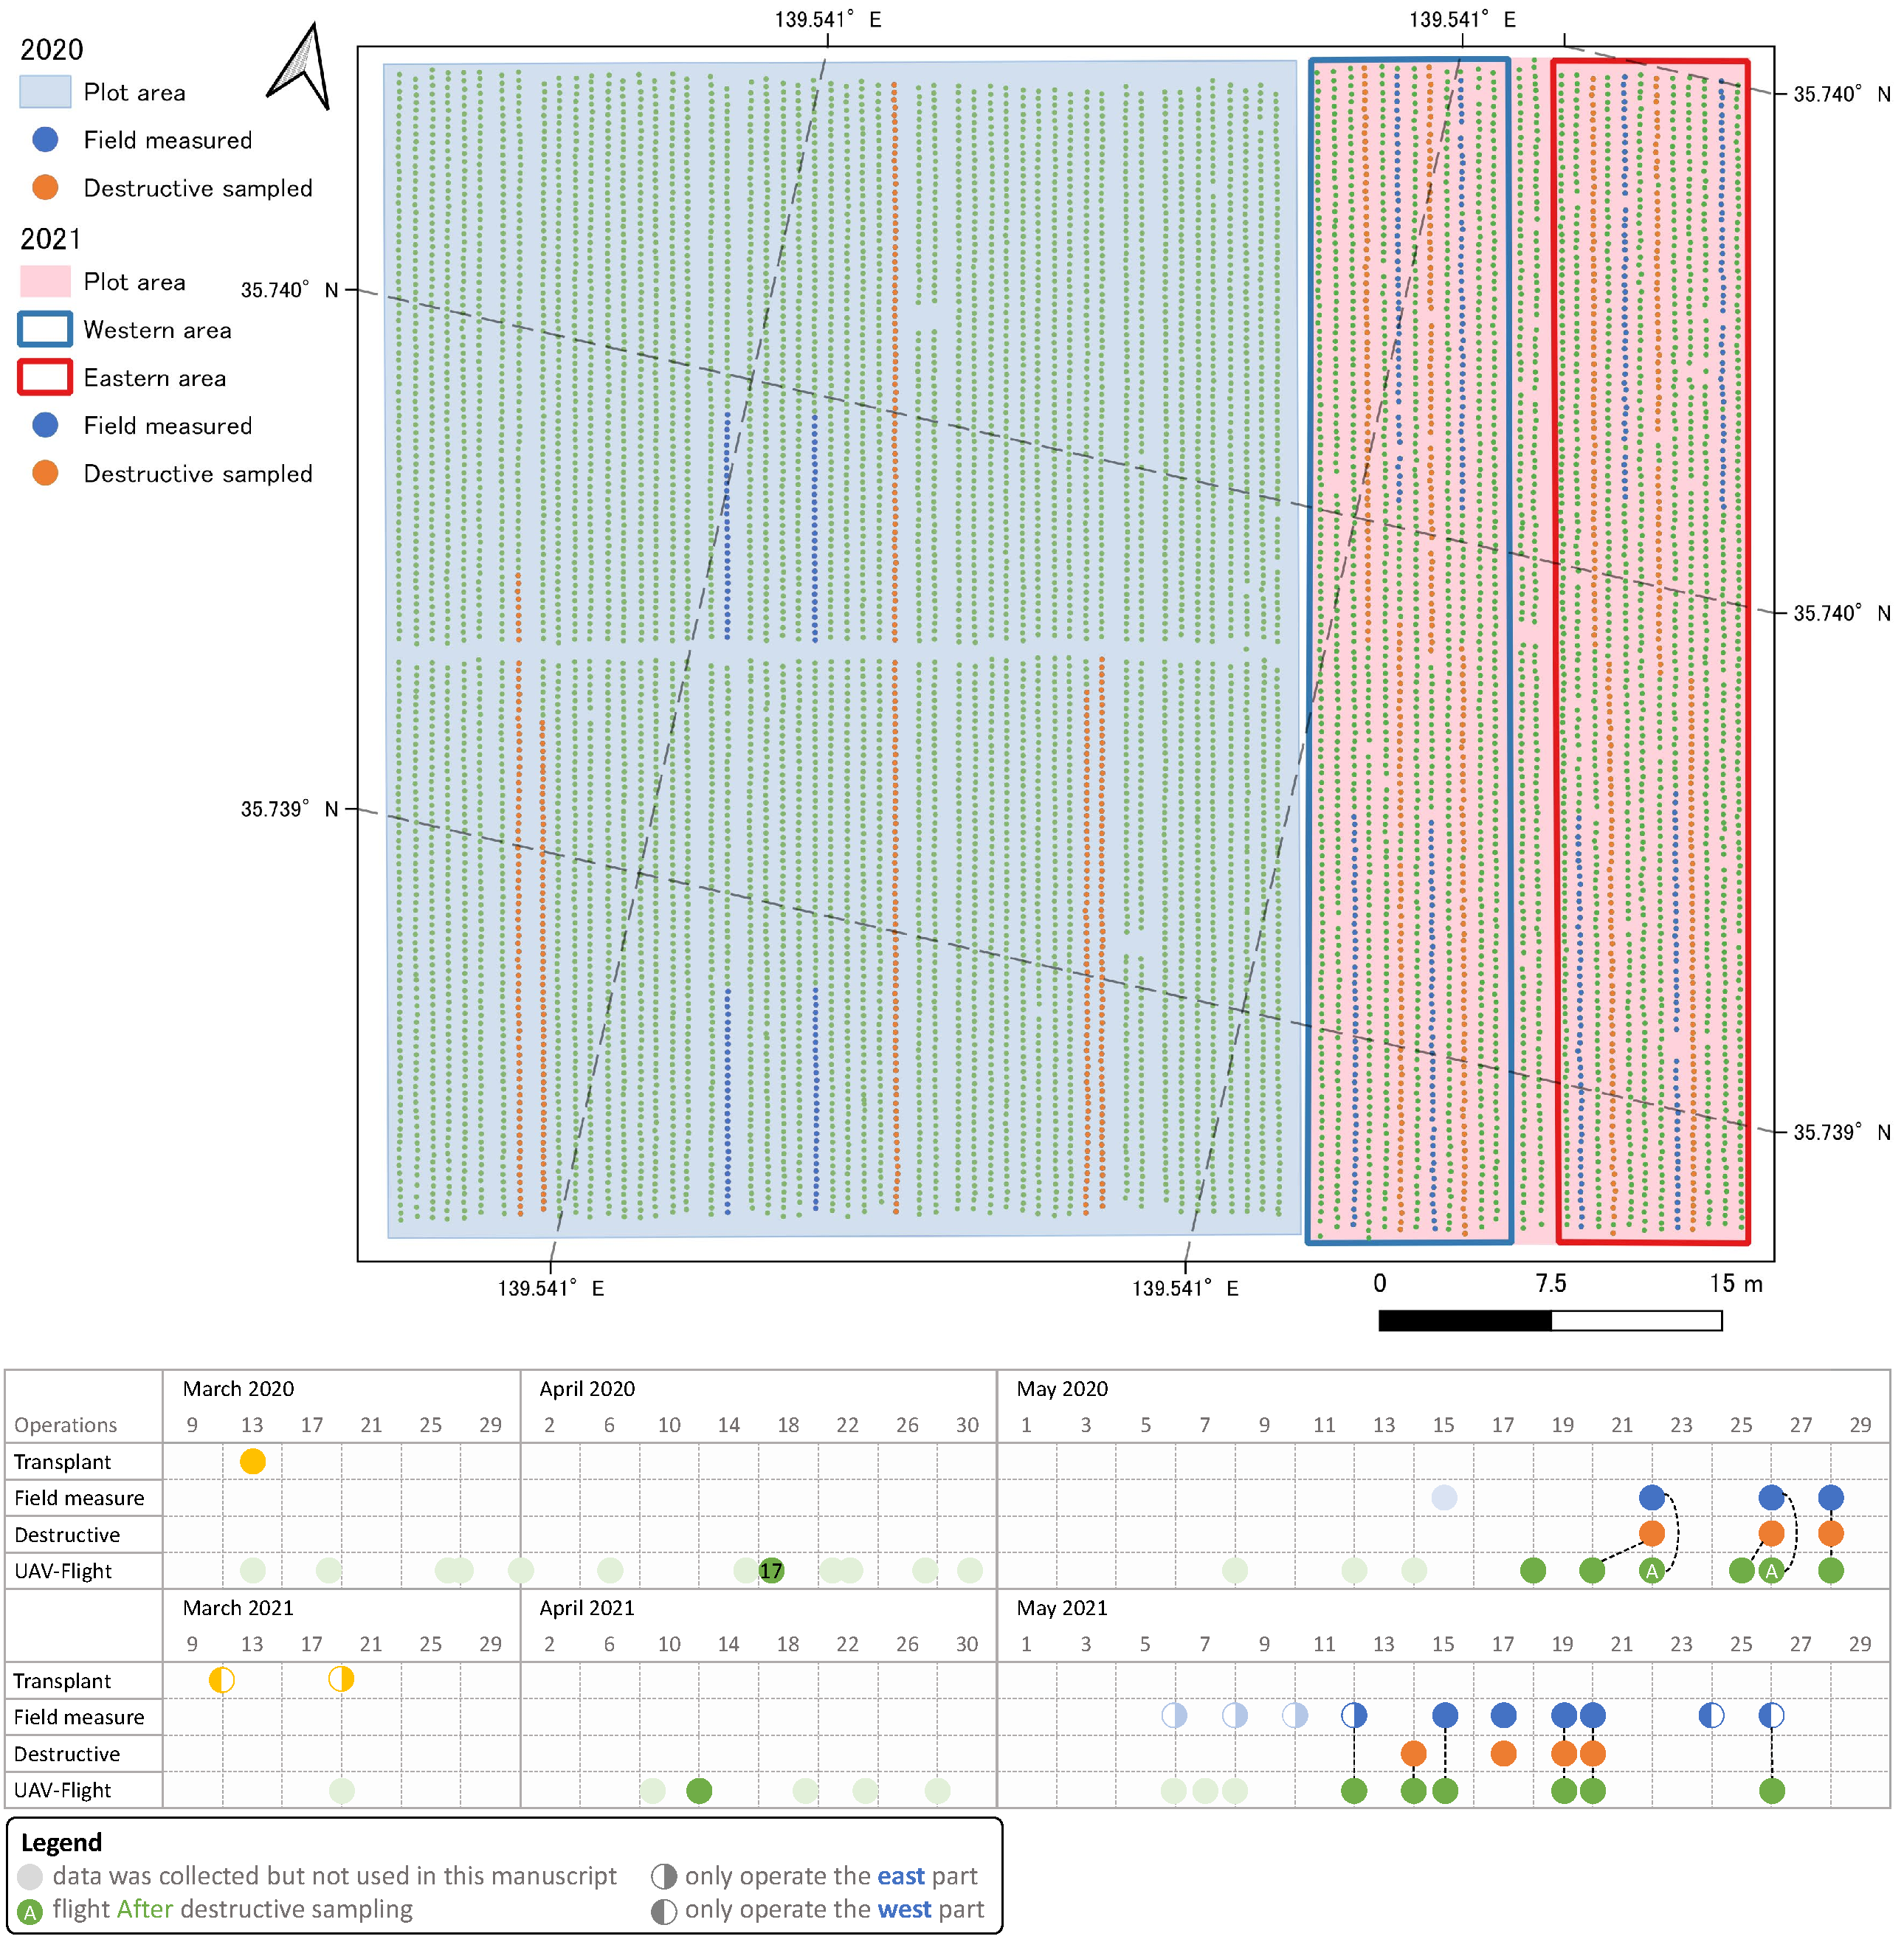
\includegraphics{figures/bro/Fig.5_data_collection_flowchart.pdf}
    }
  \end{center}
  \caption[Plot conditions and timelines for field operation and data collection]{
    Plot conditions and timelines for field operation and data collection. The plots are connected but do not have overlap for both years. Field operations include transplanting, broccoli head non-destructive measurement in the field (field measure), broccoli head destructive measurement, and UAV field investigation. In the field map, the field measurements were conducted on the fixed blue positions on every occasion, whereas the orange positions were the final of all destructively sampled positions. In the timeline, the broken dash line demonstrates how these data were paired.
  }
  \label{fig:bro5}
\end{figure}

The field data of the broccoli head size were measured as validation data (ground truth). This was conducted manually every 2‒3 d using both destructive and non-destructive measurement methods. Non-destructive measures were conducted directly in the field and destructive measures were conducted indoors. In 2020, the maximum broccoli head length was measured by the visual judgment of the longest axis. A total of $120 \times 3$ non-destructive and 434 destructive measurements of 7438 individual broccoli were recorded. 

In 2020, we identified the potential of the proposed algorithm. To further validate this algorithm, we improved the measurement method and increased the number of field samples in 2021. The maximum head length was measured using the maximum value of the length in the $0^\circ$, $45^\circ$, $90^\circ$, and $135^\circ$ directions. To increase the variation in the broccoli head for each survey, there was an 8-day interval between seeding in the western and eastern parts (timeline in Fig.~\ref{fig:bro5}, yellow lunar phase). A total of 2,000 ($400 \times 5$) non-destructive and 557 destructive measurements of 3276 individual broccoli were recorded. To reduce the workload, only half of the area (east or west) was measured on a certain day (timeline in Fig.~\ref{fig:bro5}, blue lunar phase). Head length measurements ranged from 2‒25 cm.

\subsection{Data collection and preprocessing}

After transplanting, several ground control points (GCPs) boards were set at the four corners and within the field for UAV data collection. This was an important resource for later 3D reconstruction and time-series alignment. In this study, all GCPs were measured using hemisphere Real Time Kinematic (RTK) differential GNSS devices to obtain geographical coordinates. However, it is recommended but not mandatory. For developing regions without RTK services, the GCPs' coordinates can be replaced by measuring distances (as scalebar corrector) among each GCP and building a referencing map at the very beginning. The relative coordinates of those GCPs on the referencing map can function the same as the actual geographic coordinates for time-series alignment.

Aerial images were collected using a DJI (SZ DJI Technology Co., Ltd. China) Phantom 4 v2 (camera model FC6310s), a DJI Mavic 2 Pro (camera model Hasselblad) in 2020, and a DJI Phantom 4 RTK (camera model FC6310R) in 2021. The image resolution was the same at $5472 \times 3648$ pixels. The flight height in 2020 was initially 15 m and then decreased to 10 m when the broccoli head turned up. The flight height in 2021 was constantly 15 m. Most of the flights were conducted before the field operation, except on May 22 and 26, 2020. On both these days, the destructively sampled broccoli did not exist in the UAV image; hence, the destructive data were linked to the previous flight (the black broken lines in the timeline in Fig.~\ref{fig:bro5}). For all other times, data collected on the same day were paired together.

The configuration of the computer for 3D reconstruction was as follows: Intel CITM, i9-7980XE CPU \@2.6GHz, 64GB RAM, two NVIDIA GeForce GTX 1080Ti GPUS, and Windows 10 Pro 64-bit operating system. Pix4DMapper Pro (Pix4D, S.A., Prilly, Switzerland) was used to perform flight investigations. The default software parameters were used and the GCPs were marked manually on the closest 3‒5 images. The reconstruction parameters, digital orthophoto map (DOM), and digital surface model (DSM) were produced for later use. 

The open-source software package QGIS (\url{www.qgis.org}) was used to prepare and modify GIS shapefiles, such as field boundaries and field grids on the field map (DOM). The field boundary (plot area) was a rectangular region that tightly wrapped around the broccoli (Fig.~\ref{fig:bro5}). It could be used to filter the noise outside the broccoli plot. The long boundary edges were parallel to the ridge direction (Figs.~\ref{fig:bro5} and ~\ref{fig:bro6}b). Grid plots (yellow squares in Fig.~\ref{fig:bro6}b) shared the same direction as that of the broccoli ridge and overlapped the boundary. For each grid, the edge length was 2.5 m (approximately 1000‒1500 pixels) and contained approximately 50‒100 broccolis. 

\begin{figure}[htb]
  \begin{center}
    \resizebox{\textwidth}{!}{
      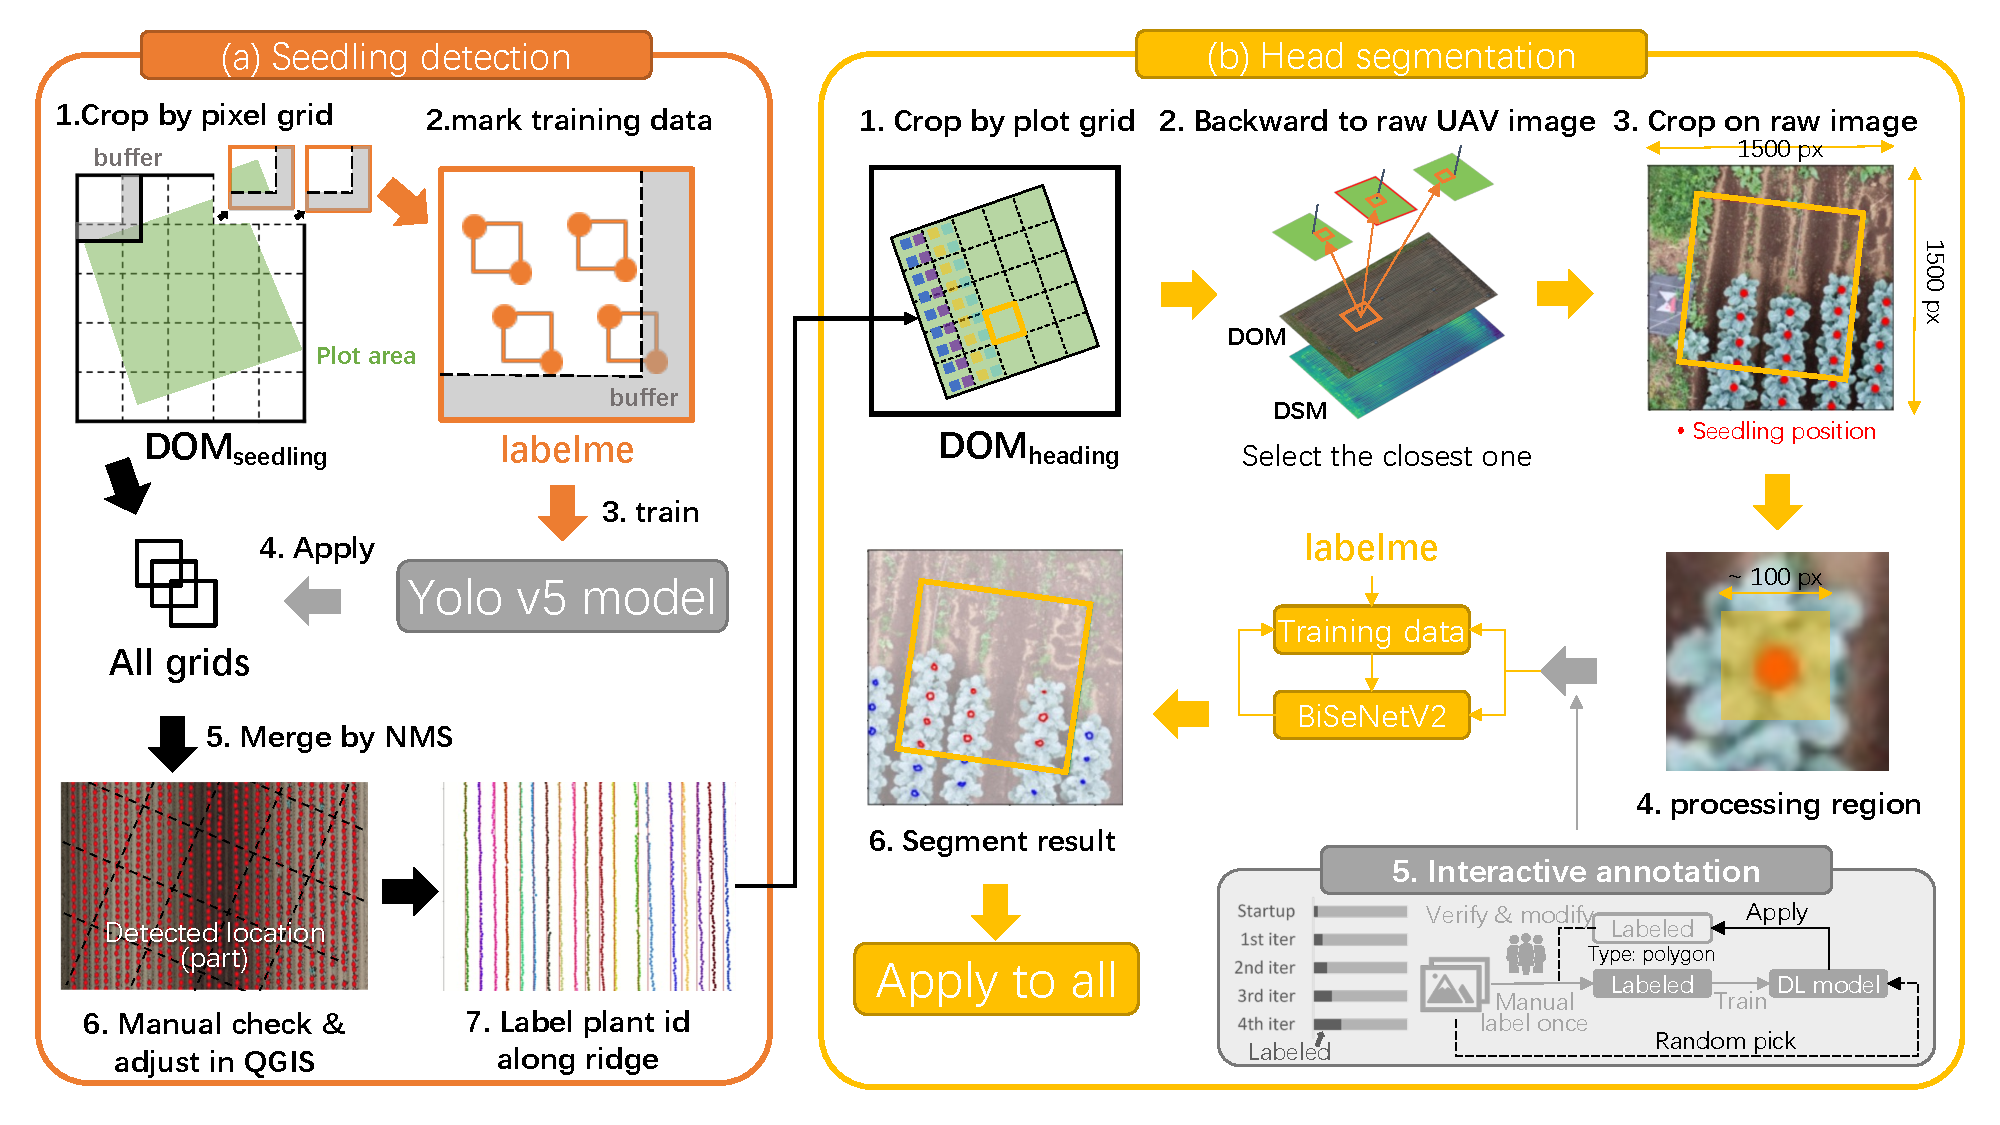
\includegraphics{figures/bro/Fig.6_dl_workflow.pdf}
    }
  \end{center}
  \caption[Workflow of broccoli seedling detection and head segmentation]{
    Workflow of broccoli (a) seedling detection and (b) head segmentation.
  }
  \label{fig:bro6}
\end{figure}

The LabelMe annotation tool (\url{https://github.com/wkentaro/labelme}) was used to label the training data for the deep learning models. EasyIDP \citep[\url{https://github.com/UTokyo-FieldPhenomics-Lab/EasyIDP}]{wang_easyidp_2021} was used to locate and crop the same field region imagery on the original UAV images when the DOM was not sufficiently clear for head segmentation (also known as backward projection or reverse calculation).

\subsection{Seedling position detection}

The difficulty of detection varied throughout the broccoli growth season. Detection during the seedling stage was simpler than that during the flowering stage, and the latter had complex leaf occlusion. The seedling position of the broccoli was almost the same as that of the broccoli head. Aligned by the GCPs, the positions were consistent through the time-series DOM and DSM of the full growing season. The results from the easy task of detecting the position in the early stage could be directly used for the subsequent complex flower stage (pre-position-guided). This significantly decreased the difficulty and workload of data analysis for broccoli head analysis.

The flight at approximately 1 month after transplanting was used to detect seedling positions (Fig.~\ref{fig:bro5}, dark green circle in April). During this period, most broccoli leaves were sufficiently large to be clearly observed from the DOM, but the leaves were not connected to each other. The uniform light conditions and differentiation between leaves and backgrounds were also taken into consideration when selecting the most suitable detection time.

The broccoli detection procedure is illustrated in Fig~\ref{fig:bro6}a. The full DOM was first split into several small pixel grids (named `sectors', Fig.~\ref{fig:bro6}a) along the DOM pixel matrix as the input of YOLO v5 (\url{https://github.com/ultralytics/yolov5}) by EasyIDP. The edge length of each sector was 1300 pixels and was buffered with 200 pixels (gray L-shape in Fig.~\ref{fig:bro6}a) on the lower right corner ($1300 \times 1300$ to $1500 \times 1500$) to avoid individual division on sector edges. Training data with only two sectors were labeled using LabelMe (Fig.~\ref{fig:bro6}a). 

Subsequently, the YOLO v5 detection model with default settings was trained and applied to all sectors. Outliers and noise outside the broccoli field were filtered by the plot area boundary. The duplicated buffer zone detection results were merged using the non-maximum suppression (NMS) algorithm. The center point of the bounding box was then viewed as the broccoli position. Finally, we manually inspected and adjusted the results in QGIS, ensuring no missing or duplicate detections (Fig.~\ref{fig:bro6}a). The broccoli ID was given from the north to the south of each ridge and ridges from the west to the east by the ridge detection algorithm (Fig.~\ref{fig:bro6}a; please refer to the links in the data availability section for further details). 

\subsection{Broccoli head segmentation}

Leaf movement and occlusion often cause DOM with double mapping, excessive pixelation, and seamline distortions \citep{lin_new_2021}. It is difficult to obtain a DOM that meets the consistent quality of the full field for head size estimation. To manage this situation, the same region on the raw UAV images (rather than that on the DOM) was used for analysis by backward projection \citep{wang_easyidp_2021}, please check the supplemetary material \ref{spp:backward} backward projection methodology for more details. To reduce the workload of segmentation model training, only the area around the broccoli seedling positions was used. Meanwhile, interactive annotation (also referred to as active learning-inspired annotation \citep{ghosal_weakly_2019}) was applied to decrease the workload of label annotation. The workflow is illustrated in Fig.~\ref{fig:bro6}b.

For image data preparation, only flights with visible broccoli heads were chosen for all 12 flight investigations over 2 years (Fig.~\ref{fig:bro5}, dark green circles in Mays). The plot area was divided into grids. For each grid, the grid boundary and broccoli positions were backward-projected onto the closest raw aerial image (Fig.~\ref{fig:bro6}b). Each raw aerial image was cropped into small sectors ($1500 \times 1500$ px) which were located in the center and contained broccoli seedling positions (Fig.~\ref{fig:bro6}b). Only the square area (approximately 100px side length) buffered from the seedling positions was used for broccoli head segmentation (Fig.~\ref{fig:bro6}b) to eliminate the effects of soil and weeds.

Considering the promptness of the interactive annotation, BiSeNet v2 \citep{yu_bisenet_2020} was used as the segmentation model. BiSeNet v2 is a network structure that employs multiple branches to process inputs of different sizes to strike a balance between the efficiency and computational cost \citep[Fig.~1]{yu_bisenet_2020}. The BiSeNetV2 network used in the present study was based on the \url{https://github.com/CoinCheung/BiSeNet} GitHub project. Our data augmentation strategy used both geometric (G) and photometric (P) transformations, similar to \citet{blok_effect_2021}. The G strategy consisted of \textit{ShiftScaleRotate} (shift limit = 0.5, scale limit = 0.2, rotate limit = 90) and \textit{VerticalFlip}, which were used to solve the problem caused by our point-based or position-guided segmentation workflow. Ideally, the input images had only one broccoli in the middle of the input image, but in actual practice, the broccoli head position appeared randomly caused by bud-head growth shifting, or even with the probability of multiple or no broccoli heads in the input images. The P strategy simulated ``cloudy, sunny" and ``day, night" transitions using RGB shift (r shift limit = 25, g shift limit = 25, b shift limit = 25) and \textit{RandomBrightnessContrast} (brightness limit = 0.3, contrast limit = 0.3) to address the effects of different weather and light conditions due to different flight investigations.

Interactive annotation was used to decrease the workload of image labeling \linebreak (Fig.~\ref{fig:bro6}b). Initially, a small number of startup training data (approximately five to ten broccoli heads per flight) were manually marked using LabelMe; then, the segmentation model was trained using the startup data. Next, images were randomly selected and applied to the segmentation results. These results were transformed into LabelMe JSON formats using Python scripts. Subsequently, manual adjustment produced annotations as new training data in LabelMe. The previous steps were iteratively repeated until no significant adjustment was required for the newly applied results.

The verification dataset for the model performance evaluation was also prepared using the previous interactive annotation. The modified intersection of union (IoU) was used as the evaluation metric. In this case, only the segmentation results inside the grid region (Fig.~\ref{fig:bro6}b, red polygon inside the yellow square) were chosen as the final results. The segmentation results attached to the grid bottom and right edge were also removed because of duplication with the neighboring grids. Here, we renamed the modified IoU inside the grid region as ``mid-IoU" (middle IoU).

The segmentation model was first trained using only the 2020 dataset for several iterations until a good performance was achieved. The model was then applied to the 2021 dataset over several iterations. When the model performed well in both years, it was applied to all dataset images, and the segmentation results after the grid boundary filter were saved for the next procedure.

\subsection{Head traits calculation}

The unit of the segmentation polygon in raw aerial images was a pixel, which could not represent the actual head size. However, the actual head size could be calculated using the pixel scale bar from the geo-referenced DOM. The pixel scalebar on the raw images could be derived from the ratio between the grid size in pixels on the raw image and that on the DOM. This concept was then implemented using projective transformation in scikit-image (\url{https://scikit-image.org}). On some locations, one broccoli may have had duplicated polygons; only the polygon with the largest area was retained, which was accelerated by a k-dimensional tree (KD-Tree) in SciPy (\url{https://scipy.org}).

For each polygon of broccoli head, the following geometry traits were calculated: 1) max length and min length, from the side lengths of the minimum area bounding box; 2) perimeter, circularity and area of polygon; 3) area of polygon convex hull; 4) major length, minor length and eccentricity of ellipse has the same second-moments as the polygon. 5) equivalent diameter of circle has the same area as the polygon.

\subsection{Field validation for head traits}

To test the correlation between field-measured length (dependent variable) and aerial measured length (independent variable), the coefficient of determination ($r^2$) using simple linear regression was used as the evaluator. To assess the trends in differences in broccoli size in detail, locally weighted scatterplot smoothing (LOWESS) regression and distribution comparison were also used.

\section{Results}

\subsection{Broccoli position detection}

To provide a general understanding of this procedure, Supplementary Figs.~\ref{fig:bros1}a to f shows some intermediate results during broccoli position detection. As mentioned in the Materials and Methods section, the DOM of the entire broccoli plot was first divided into several small sectors with a buffer zone. For training data preparation, considering the significant differences between the broccoli plant and brown soil, only two representative sectors were chosen as training images. All broccoli were labeled using bounding box (rectangle) annotation in LabelMe (Supplementary Fig.~\ref{fig:bros1}a, example sector). The detection model performed as expected in the other sectors (Supplementary Fig.~\ref{fig:bros1}b: one example sector). The green mask in Supplementary Fig.~\ref{fig:bros1}b shows the buffer zone that overlapped with neighboring sectors, with the aim of avoiding incomplete broccoli detection on the sector boundary. When merging the detection results for all sectors, duplicate detections were removed by the NMS algorithm (black rectangles in Supplementary Fig.~\ref{fig:bros1}c). When adjusting the zoom to the full map view, the removed black duplicates were clearly distributed on the sector boundaries (grid lines). The center of the detected bounding box was viewed as the broccoli position; however, it required manual inspections to correct false detections and missing broccoli. In Supplementary Fig.~\ref{fig:bros1}d, the green dots show the manually corrected (removed) YOLO detection results, and the red dots indicate the final positions used by manual adjustment. Supplementary Figure~\ref{fig:bros1}e shows the results of ridge-line detection, and Supplementary Fig.~\ref{fig:bros1}f shows some results of the automatic broccoli ID assignment. In general, broccoli position detection and semi-automatic labeling functioned as expected.

\subsection{Broccoli head segmentation}

To clearly demonstrate the interactive annotation procedure, Supplementary \linebreak Figs.~\ref{fig:bros1}g to i and Supplementary Table~\ref{tbl:bros1} provide example images and a simple summary from the first to the last iteration. As startup training data, one image was randomly selected from each flight investigation in 2020, and only a few representative broccoli were annotated as simply as possible (Supplementary Fig.~\ref{fig:bros1}g). The BiSeNet model (v0) was then trained using this annotation. For each flight in 2020, one image was randomly selected and applied to the v0 model (Supplementary Fig.~\ref{fig:bros1}h, red mask). The results were manually adjusted and saved as new training data (Supplementary Fig.~\ref{fig:bros1}h, blue boundary). The previous steps were iteratively repeated until the model achieved good segmentation results, and this version (in this case, v2) was used to produce 30 validation data with low labor costs. The model performance was evaluated using validation data.

The detailed model performance for each iteration version is presented in Supplementary Table~\ref{tbl:bros1}. With the proposed guidance of the broccoli position and the buffered mask, even a startup with only a few annotations could achieve a mid-IoU of 78.15\%. The model performance improved considerably after four iterations and achieved a mid-IoU of 88.33\% after the 4th iteration (Supplementary Fig.~\ref{fig:bros1}i). Then, when the v4 model trained by 2020 data was applied to the 2021 data, the performance decreased to 79.16\%, as expected. However, it significantly improved to 91.70\% after one additional iteration with six training data points added from 2021. Meanwhile, broccoli head segmentation was more challenging at an early stage (May 18, 2020, and May 12, 2021, with the lowest mid IoU) when the head size was small. This suggested that weakly supervised annotation improved the model performance and decreased the workload in data annotation with iteration.

\subsection{HD validation}

The full map of all calculated HDs from the UAV is shown in Supplementary Fig.~\ref{fig:bros2}. We found a high correlation between the maximum length of the broccoli head measured by the UAV image and that measured manually in the field (Fig.~\ref{fig:bro1}). The UAV method tended to underestimate broccoli growth (trend line above the reference line). However, the overall distribution of the estimated head size was almost the same between the two groups (UAV vs. manual, Figs.~\ref{fig:bro1}c and d). 

\begin{figure}[htb]
  \begin{center}
    \resizebox{\textwidth}{!}{
      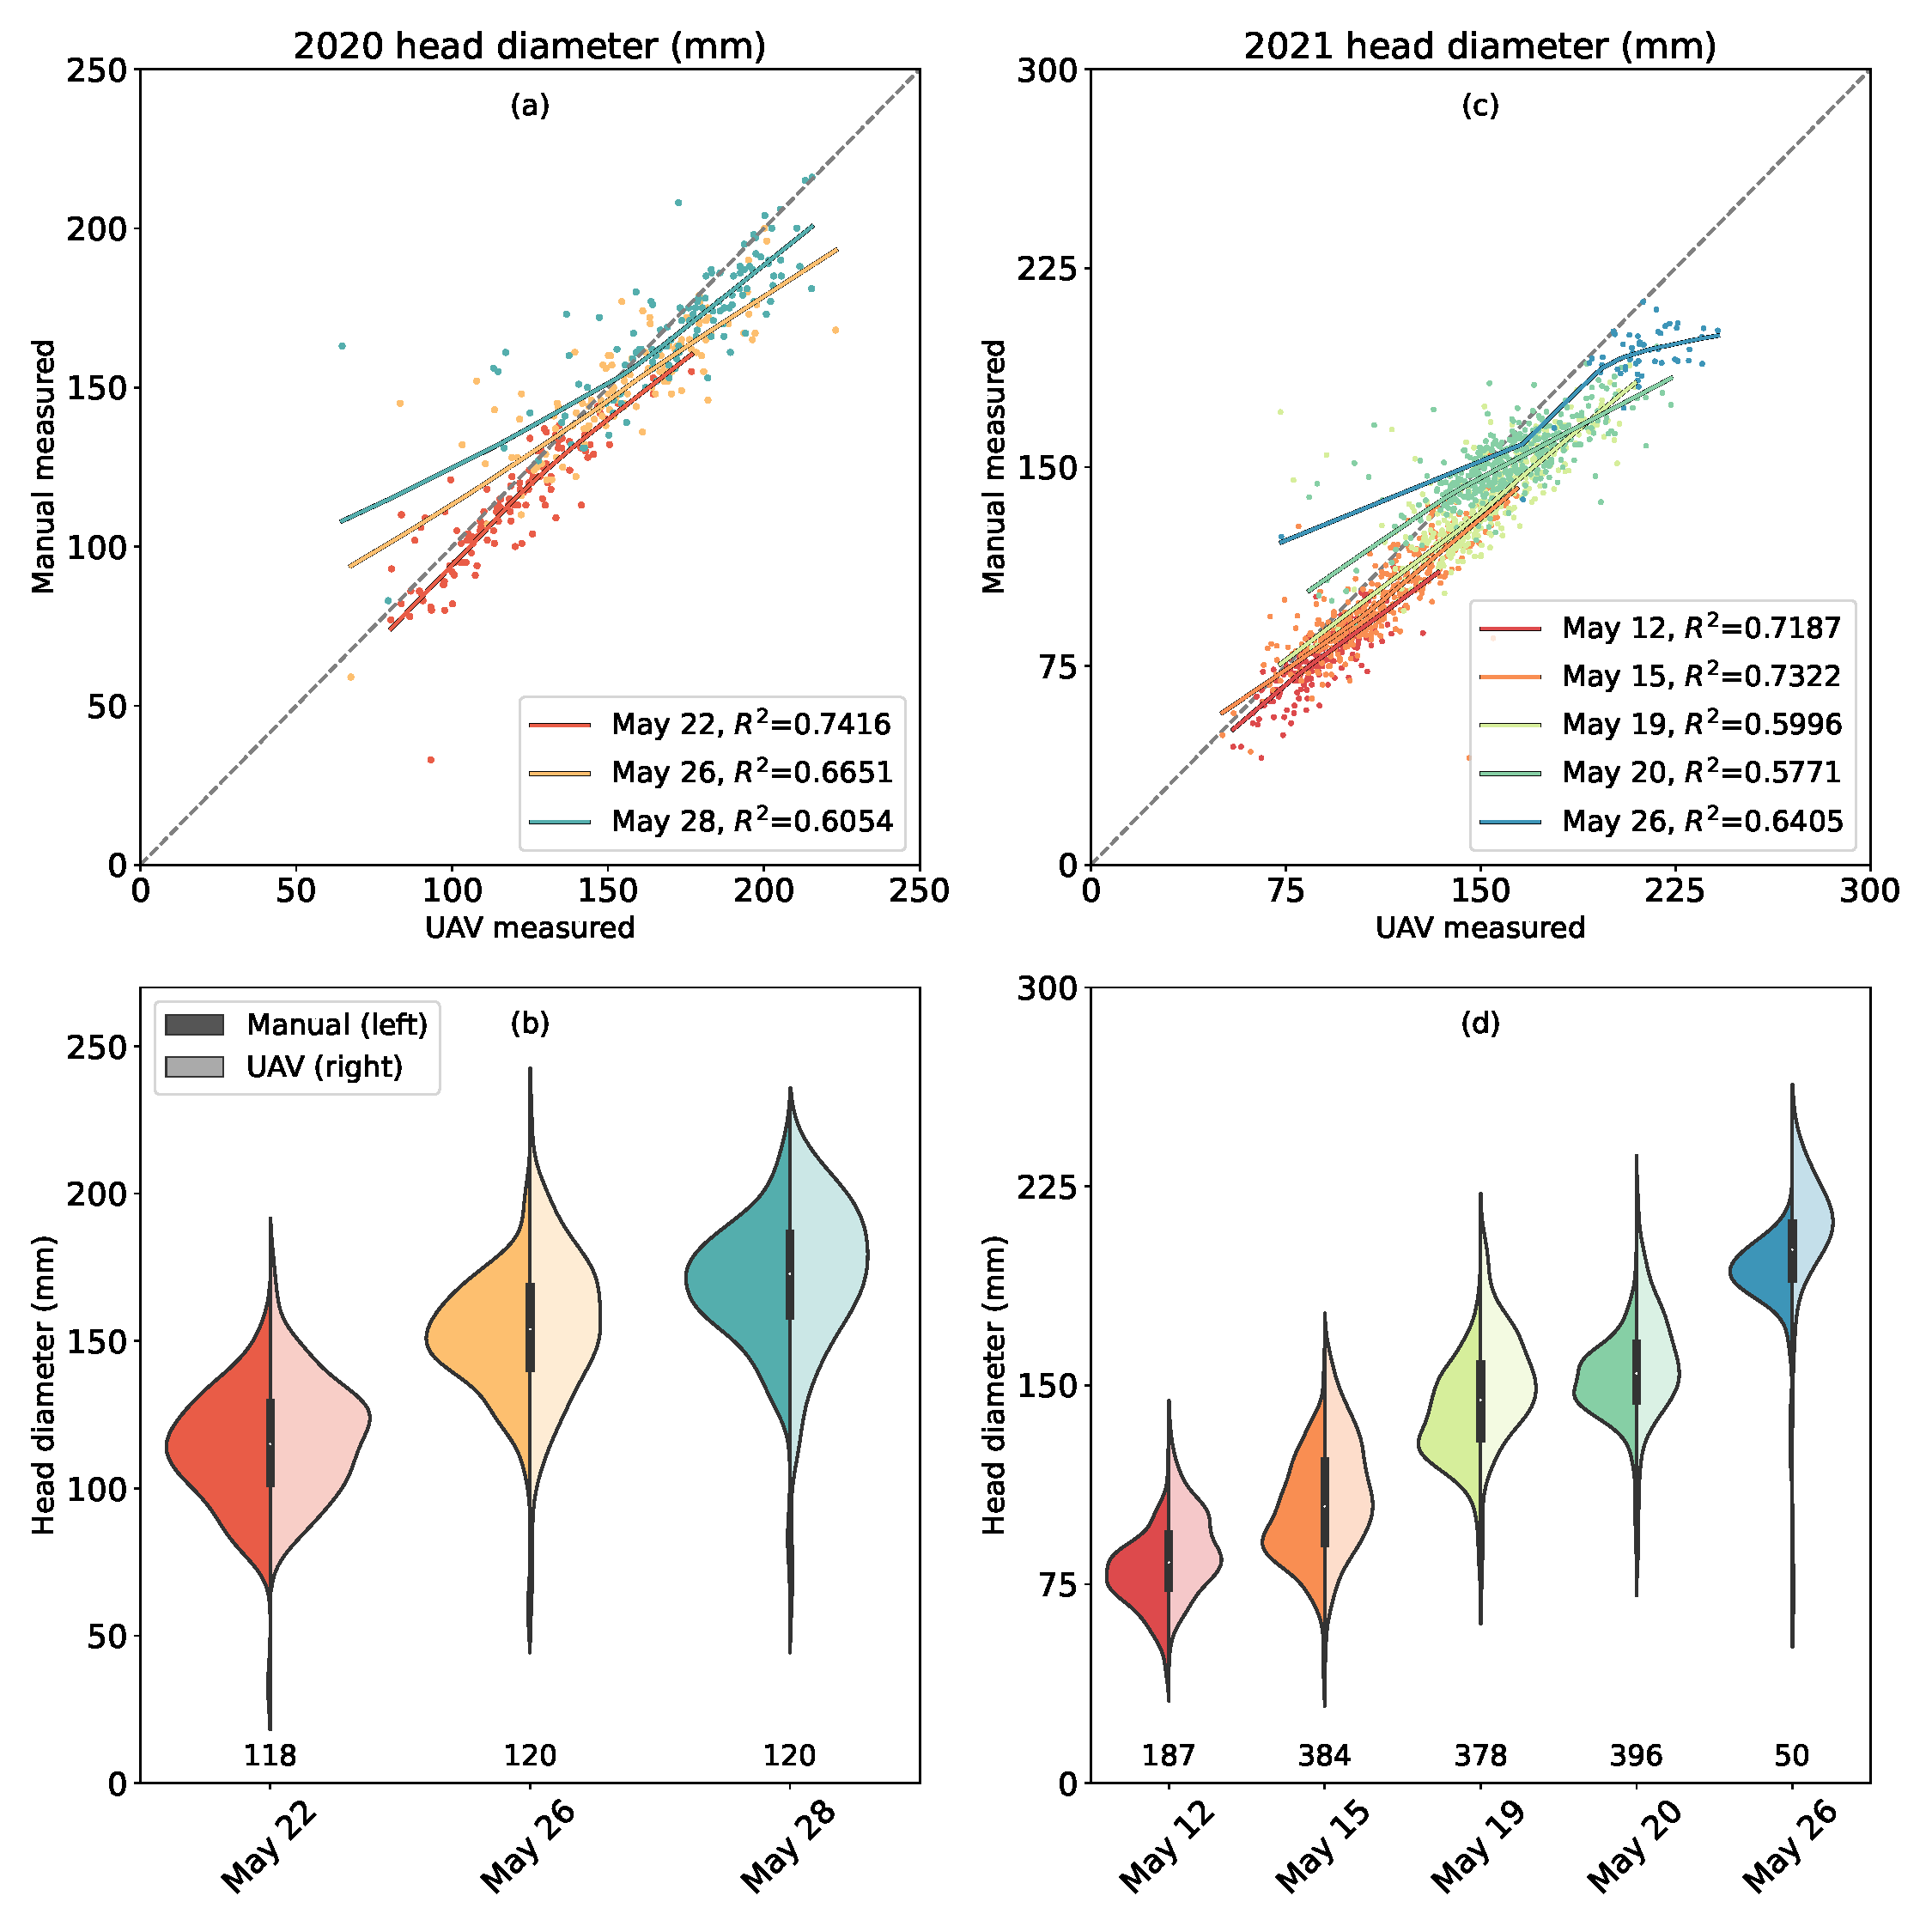
\includegraphics{figures/bro/Fig.1_compare_merge_230207.pdf}
    }
  \end{center}
  \caption[Comparison of broccoli head diameter measured from UAV images and obtained using manual field measurements]{
    Comparison of broccoli head diameter measured from UAV images and obtained using manual field measurements. Different colors represent different investigation dates. 
    In (a) and (c), the curved solid lines represent the trends by locally weighted scatterplot smoothing (LOWESS) regression. 
    In (b) and (d), the violin plots show comparisons of the value distribution; 
    darker colors (left part) show manual field measurements, brighter colors (right part) show UAV measurements, and the values below show the broccoli count.
  }
  \label{fig:bro1}
\end{figure}


\section{Discussion}

Reducing on-farm food loss (e.g., non-standard-sized vegetables) is one of the prominent goals of sustainable development in agricultural production. The main aim of this work is to test the use of UAV-mounted digital measurements of broccoli head size and their use in monitoring for different sellable size classes. In this study, we created a broccoli head size estimating pipeline based on UAV imagery, machine learning / deep learning (ML/DL) in the entire broccoli field. Our experiments demonstrated that the head sizes estimated by UAV imagery were highly correlated with the field measurements. Although the current study focused on broccoli as a model system, this framework could be readily applied to other similar vegetables such as cauliflower, artichoke, and cabbage. Thus, our case study shows that smart farming techniques have great potential to contribute to the sustainable development of vegetable production.
% Reducing on-farm food loss (e.g., non-standard-sized vegetables) is one of the prominent goals of sustainable development in agricultural production. The main aim of this work is to test the use of UAV-mounted digital measurements of broccoli head size and their use in monitoring and prediction of optimal harvest time in terms of economic returns for different sellable size classes. In this study, we created a harvest date prediction system based on UAV imagery, machine learning / deep learning (ML/DL), and a growth model by predicting the short-term change in the head size of all individuals ($> 3000$) in the entire broccoli field. Our experiments demonstrated that: (1) the head sizes estimated by UAV imagery were highly correlated with the field measurements; (2) the proportion of non-standard-size and the total income calculated by the hypothetical harvesting changed dramatically between harvest days; (3) predictions for the few days following a particular date of UAV imagery were highly correlated with those estimated by UAV imagery taken on that date; and (4) the optimal harvest date (i.e., the date for the minimum proportion of non-standard-size broccoli and maximum income) could be predicted with high accuracy. These results suggested that our prediction system for the optimal harvest date of broccoli will benefit farmers by reducing food loss and increasing their income. Although the current study focused on broccoli as a model system, this framework could be readily applied to other similar vegetables such as cauliflower, artichoke, and cabbage. Thus, our case study shows that smart farming techniques have great potential to contribute to the sustainable development of vegetable production.

% This study showed that the proportion of non-standard-size broccoli and the total income changed rapidly depending on the harvest date. For example, 1 day later or earlier than the optimal harvest date increased the number of non-standard-size broccoli by approximately 5\% and decreased the total income by approximately 20\%; and 2 days later than the optimal harvest date increased the number of non-standard-size broccoli by approximately 15\% and decreased the total profit by approximately 40\%. To the best of our knowledge, such temporal changes in the number of non-standard-size vegetables and the total profit for different harvest dates have not previously been calculated because no technique was available to measure thousands of individual vegetables multiple times with high accuracy. Interestingly, the optimal harvest date was largely unaffected by differences in the shipping price for each grade (Figs.~\ref{fig:bro3}c and d). The optimal harvest date was determined by the spatial variation in broccoli growth, regardless of the shipping price of each grade. The difficulty in setting the harvest date for mechanical harvesting owing to large spatial variation is a common issue in broccoli and other vegetable farms. Thus, predicting the optimal harvest date using our system (or similar systems) has the potential to reduce on-farm food loss and increase the income of vegetable farmers worldwide.

In addition to estimating temporal variations in head size distribution, our pipeline could visualize spatial variations in individual head size (Supplementary Fig.~\ref{fig:bros2}). In the 2021 trial, spatial variation in broccoli size was intentionally created by planting seedlings on two different dates in the eastern and western areas of the field (8 days intervals). When we visualized the individual head sizes, the difference between the eastern and western fields was evident. However, it was difficult to visually observe the differences on the ground. For example, the difference in average head size between the east and west on March 12, 2021, was only 3 cm. Although the uneven growth between the west and east fields in this trial was intentional, such spatial variation can occur unintentionally and is a major challenge, especially in large-scale agriculture \citep{quine_investigation_2002}. In such a large-scale uneven field, farmers can divide their field into several areas and harvest broccoli multiple times. Using our framework, farmers may be able to visualize the spatial variation of their fields, predict their short-term growth, and determine the optimal spatial and temporal harvest strategy.

Although our developed system highlights the benefits and importance of UAV imagery powered by ML/DL for sustainable agricultural development, there are some limitations to its use. First, our system is neither fully automated nor app-based; therefore, farmers without computer science backgrounds cannot use this system directly in their fields. However, because the source code is open to the public (\url{https://github.com/UTokyo-FieldPhenomics-Lab/UAVbroccoli}), local agricultural institutes and agricultural companies will be able to modify and use the system according to their target vegetables and varieties. This study is definitely not a one-stop solution, but as a pioneer to solve the zero-to-one problem in real agriculture production. Second, unlike the traditional method conducted by sampling measurement, the proposed method is based on the time-series per-crop investigation. Such high-throughput phenotyping data could power the data-driven model to a new level. Third, manual inspection of the seedling position detection results is required; this step cannot be omitted because this result is the basis for subsequent broccoli segmentation. Detection omissions, duplications, and drifts need to be checked manually on a case-by-case basis. Although it saves considerable effort compared to adding them manually one by one, this inspection still requires several hours to complete in large-scale fields. Fourth, the problem of leaf occlusion has not been solved, which remains a challenging problem for plant phenotyping \citep{zhang_applications_2020}. As broccoli heads are essentially round, one approach is to restore the roundness of the stubs. The circularity and eccentricity of the broccoli head may be used to describe the severity of occlusion. The least squares for round fitting can be used, or the deep learning framework ORCNN can be applied to obtain improved recovery results \citep{blok_image_2021}. However, it requires a depth camera and image pairs before and after occlusion as training data is collected on the ground, which is inconvenient for current UAV applications but warrants further study. For example, multi-spectral and even LiDAR sensors are becoming increasingly cheap, combined with the rapid development of AI algorithms, this problem and even this work could be refined without unaffordable cost increasing. Also, integration of the method with other commonly used agronomics practices such as mulching films with bioplastics could assist in the identification of plants and broccoli heads, particularly when used in conjunction with a multi-spectral sensor. Finally, hardware and software instrument costs should not be omitted. In this study, the UAV with RTK (\$6,500), 3D reconstruction software (\$3,499), and a high-performance computer (\$6,000) for computation limit its widespread use for single farmers. However, even for a small farm (0.2 ha) with 7,000 broccoli plants, only 2 days difference from the optimal harvest date can result in an income loss of almost \$2,000. Larger farms are worth investigating in the future. For companies that provide this type of agricultural consulting service, this one-off investment can be offset by the increased profit in a short time. For those economically and socially disadvantaged rural regions, the RTK or the expense of a base-station is not mandatory. It can be replaced by setting more GCP boards and measuring distances among them as scalebar correctors, to get similar results with relative geographical coordinates. For future work, we will cooperate with local broccoli farmlands to test the proposed system without RTK dependences, and keep improving the algorithm performance on the occlusion area as discussed before. The head quality and transport costs will also be integrated into the system to refine its applicability.

\section{Conclusion}

In conclusion, this is a demonstrable application of UAV technology to assist farmers in optimizing financial returns and minimizing food waste rather than the majority of UAV / digital agriculture studies that are aspirations and lack the pipeline to actually help farmers in an applied context. In this study, using UAV imagery and ML/DL, we developed a system for estimating and predicting the head size of whole broccoli with high accuracy and showed that the system can predict the optimal harvest date. This UAV-based prediction system is based on several technical improvements and requires minimal labor and computational costs. Therefore, it could be applied to support broccoli farming, and with modifications, to a variety of similar vegetables (i.e., cabbage, cauliflower, artichoke, and lettuce). Because our developed pipeline uses a simple sensor, not a complex integration of multiple sensors, it would be more applicable and user-friendliness for economically and socially disadvantaged rural regions, and it has the potential to be widely adopted by vegetable farmers worldwide.

\hspace*{\fill}

\noindent \textbf{Acknowledgments}: We thank the technical staff of the Institute for Sustainable Agro-ecosystem Services (ISAS) for the management of broccoli fields. 

% \hspace*{\fill}

% \noindent \textbf{Author Contributions}: W.G. and Y.F. designed the study. E.N. managed the broccoli field and collected field data. W.G. (and technical staff) collected the UAV images and 3D reconstructed the plots. H.W. created the full UAV image analysis pipeline, and T.L. contributed to the deep learning and interactive annotation coding work. E.N. built the prediction models for income. H.W. and E.N. prepared the figures. H.W., E.N., and T.L. prepared the manuscript. Y.K., W.G., and Y.F. supervised this study.

\hspace*{\fill}

\noindent \textbf{Funding}: This study was partially supported by the Japan Science and Technology Agency (JST) AIP Acceleration Research (JPMJCR21U3), by the Ministry of Agriculture, Forestry and Fisheries (MAFF) ``Research project for technologies to strengthen the international competitiveness of Japan's agriculture and food industry."

% \hspace*{\fill}

% \noindent \textbf{Competing interests}: The authors declare no competing interests nor any potential conflict of interest.

\hspace*{\fill}

\noindent \textbf{Data Availability}: The source code used in this manuscript can be accessed at \url{https://github.com/UTokyo-FieldPhenomics-Lab/UAVbroccoli}. All original UAV image data can be accessed by Google Drive upon request (224GB for 2020 and 72GB for 2021). Although the data used in this manuscript were obtained using Pix4D, we updated the workflow to Metashape, which is easier for batch processing in codes since 2022.


\appendixsection

\subsection{Backward projection methodology}
\label{spp:backward}

% This section has been modified and published at the ``Remote Sensing" \citep{wang_easyidp_2021}

\begin{center}
  \noindent
  \fbox{
    \begin{minipage}{0.95\textwidth}
    
      \begin{center}
        \textbf{EasyIDP: A Python Package for Intermediate Data Processing in UAV-Based Plant Phenotyping}
      \end{center}

      \noindent Haozhou Wang$^{1}$, Yulin Duan$^{2,3}$, Yun Shi$^{2,3}$, Yoichiro Kato$^{1,4}$, Seishi Ninomiya$^{1,5}$, and Wei Guo$^{1,\star}$
    
      \noindent $^{1}$ International Field Phenomics Research Laboratory, Institute for Sustainable Agro-Ecosystem Services, Graduate School of Agricultural and Life Science, The University of Tokyo, Tokyo 188-0002, Japan;
      
      \noindent $^{2}$ Key Laboratory of Agricultural Remote Sensing, Ministry of Agriculture, Beijing 100081, China;

      \noindent $^{3}$ Institute of Agricultural Resources and Regional Planning, Chinese Academy of Agricultural Sciences, Beijing 100081, China

      \noindent $^{4}$ International Rice Research Institute, Metro Manila 1226, Philippines

      \noindent $^{5}$ Plant Phenomics Research Center, Jiangsu Collaborative Innovation Center for Modern Crop Production, Nanjing Agricultural University, Nanjing 210095, China
      
      \noindent $^{\star}$ Corresponding author

      \begin{spacing}{1.5}
      \textbf{Abstract}
      \end{spacing}
      
      Unmanned aerial vehicle (UAV) and structure from motion (SfM) photogrammetry techniques are widely used for field-based, high-throughput plant phenotyping nowadays, but some of the intermediate processes throughout the workflow remain manual. For example, geographic information system (GIS) software is used to manually assess the 2D/3D field reconstruction quality and cropping region of interests (ROIs) from the whole field. In addition, extracting phenotypic traits from raw UAV images is more competitive than directly from the digital orthomosaic (DOM). Currently, no easy-to-use tools are available to implement previous tasks for commonly used commercial SfM software, such as Pix4D and Agisoft Metashape. Hence, an open source software package called easy intermediate data processor (EasyIDP; MIT license) was developed to decrease the workload in intermediate data processing mentioned above. The functions of the proposed package include (1) an ROI cropping module, assisting in reconstruction quality assessment and cropping ROIs from the whole field, and (2) an ROI reversing module, projecting ROIs to relative raw images. The result showed that both cropping and reversing modules work as expected. Moreover, the effects of ROI height selection and reversed ROI position on raw images to reverse calculation were discussed. This tool shows great potential for decreasing workload in data annotation for machine learning applications.

      \vspace{5mm}
      \textbf{keywords}: orthomosaic; photogrammetry; phenotyping; reverse calculation; Pix4D; Agisoft Metashape; Agisoft PhotoScan

    \end{minipage}
  }
\end{center}

The function of this backward projection is projecting ROI from world coordinate to relative UAV raw images. In this section, using ``zipfile" and ``xml" Python packages to load the external and internal camera parameters generated from SfM-MVS reconstruction projects. Then apply the backward calculation using the pinhole camera model. Finally camera distortion calibration is conducted.

\subsubsection{Camera parameters loading}

The relationship between field and UAV raw images is built after running SfM-MVS software. It has two main parts, external and internal parameters. The external parameters are different for each raw image, including the camera position (x, y, z) in the real-world coordinate ($O_{world}$, Fig.~\ref{fig:idps1}.a) and the camera rotation (yaw, pitch, roll). The internal parameters describe the characteristics of the sensor and are the same as each raw image, such as focal length, camera Charge-coupled Device (CCD) size, and lens distortion calibration parameters (\url{https://support.pix4d.com/hc/en-us/articles/202559089-How-are-the-Internal-and-External-Camera-Parameters-defined}). These parameters are available under the Agisfot Metashape and Pix4D project intermediate files.

For Pix4D projects, all these parameters are located in the ``1\_initial/params" folder, the ``calibrated internal camera parameters.cam", ``calibrated camera paramters.txt", ``pmatrix.txt", and ``offset.xyz" are loaded as text directly and parsed in the EasyIDP package without any external packages. For more details about those files, please refer to the Pix4D official documentation (\url{https://support.pix4d.com/hc/en-us/articles/202559089-How-are-the-Internal-and-External-Camera-Parameters-defined}).

For Agisoft Metashape projects, all these parameters can be obtained either by calling APIs (Professional license required) or by reading zipped xml files in the project file ``project.files/0/chunks.zip/doc.xml". The EasyIDP package chose the zipped xml way without a professional license. The ``zipfile" and ``xml" packages were used to un-zip and parse these parameters in xml files.

\begin{figure}[htb]
  \begin{center}
    \resizebox{\textwidth}{!}{
      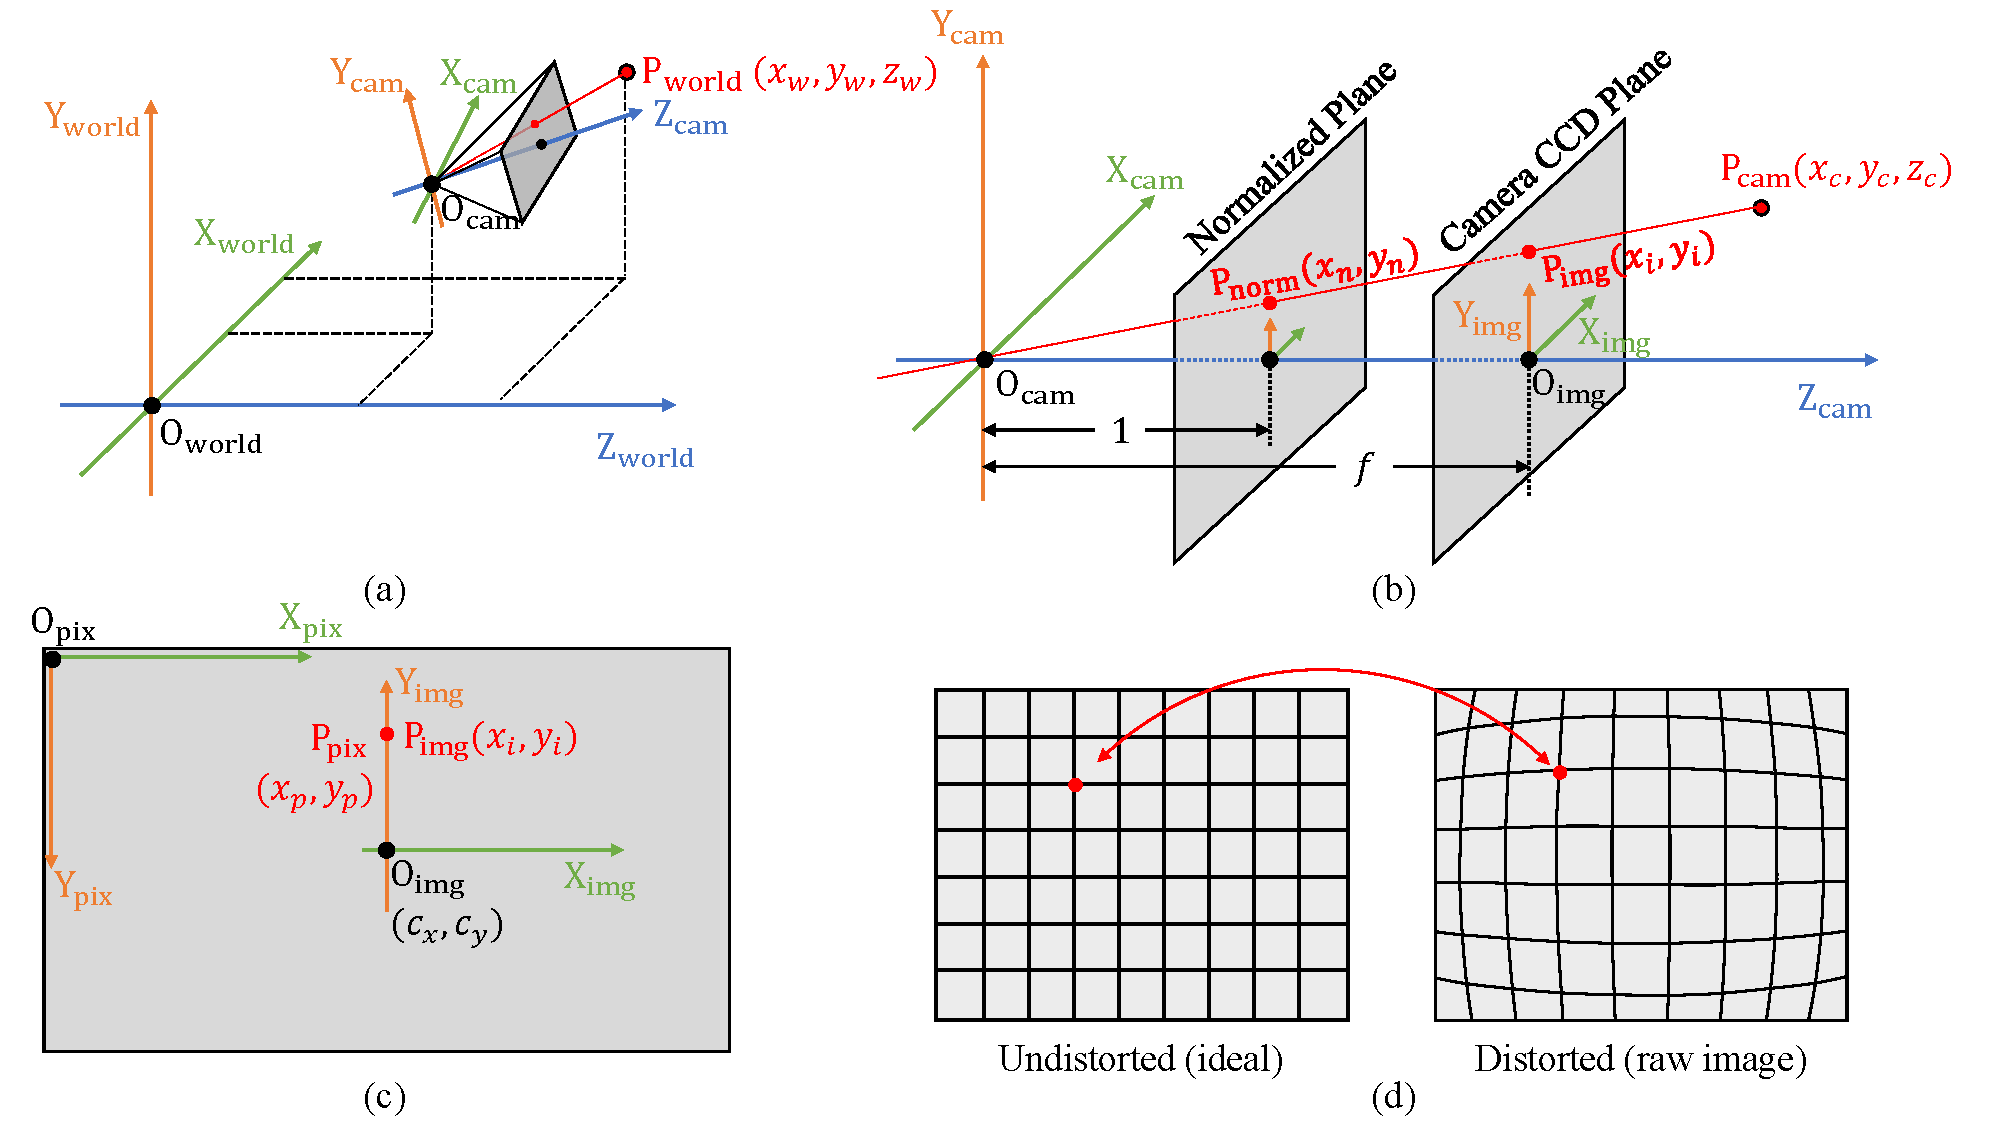
\includegraphics{figures/idp/Fig.S1_world2pixels.pdf}
    }
  \end{center}
  \caption[Backard projection illustration graph]{
     Backard projecting one point from the 3D world coordinates to the 2D pixel coordinates on raw UAV images by pinhole camera model. (a) The relationship between world coordinate ($O_{world}$) and camera coordinate ($O_{cam}$), linked by camera external parameters (position and rotation). (b) the relationship between camera coordinate ($O_{cam}$) and image coordinate ($O_[img]$). (c) The relationship between image coordinate ($O_[img]$) and pixel coordinate ($O_{pix}$). (d) The camera distortion calibration between undistorted images and distorted images caused by the lens.
  }
  \label{fig:idps1}
\end{figure}

\subsubsection{Backward projection forumulars}

The geometry from the real-world coordinate ($O_{world}$) to image pixel coordinate ($O_{pix}$) is shown in Fig. \ref{fig:idps1}.a-c. There are four coordinate systems, first is the $O_{world}$ whose unit is often meter (Fig. \ref{fig:idps1}.a). The second one is the camera coordinate ($O_{cam}$, Fig. \ref{fig:idps1}.b), which makes the camera position to the origin (0,0,0) of coordinates, and the camera optical axis is used as the z-axis (commonly, the point $O_{img}$ is not the center point of plane). The third is the camera CCD coordinate ($O_{img}$, Fig.~\ref{fig:idps1}.c) whose unit is often mm. The last one is pixel coordinate ($O_{pix}$) whose origin is the top left corner in the $O_{img}$ and the unit is pixel.

Let us assume a point $P_{world} (x_w,y_w,z_w)$ in $O_{world}$, to transform that point into $P_{cam} (x_c,y_c,z_c)$ in $O_{cam}$ (Fig.~\ref{fig:idps1}.a), the $3\times4$ transform matrix $T$ could be derived from camera position ($t$, translational transformation) and camera rotation ($R$, rotational transformation):

\begin{equation}
  \begin{array}{lll}
    P_{cam} & = & T \cdot P_{world} \\
    \begin{small}
      \left[ 
        % amsmath package is required
        \begin{matrix} 
          x_c \\
          y_c \\
          z_c \\
        \end{matrix} 
      \right] 
    \end{small}
    & = & 
      \begin{small}
      \left[ 
        % amsmath package is required
        \begin{matrix} 
          R_{11} & R_{12} & R_{13} & t_1 \\
          R_{11} & R_{12} & R_{13} & t_1  \\
          R_{11} & R_{12} & R_{13} & t_1  \\
        \end{matrix} 
      \right] 
      \left[ 
        % amsmath package is required
        \begin{matrix} 
          x_w \\
          y_w \\
          z_w \\
          1
        \end{matrix} 
      \right] 
    \end{small}
  \end{array}
\label{eq:idp1}
\end{equation}

\noindent 
Where, $t$ is the $3\times1$ position matrix, and $R$ is the $3\times3$ rotation matrix derived by $(\omega, \varphi, \kappa)$ from camera rotation parameters (yaw, pitch, roll) (\url{https://support.pix4d.com/hc/en-us/articles/202558969-Yaw-Pitch-Roll-and-Omega-Phi-Kappa-angles}):

% \begin{equation}
  \begin{array}{lll}
    R & = & R(\omega) R(\varphi) R(\kappa) \\
    & = &
      \begin{small}
      \left[ 
        % amsmath package is required
        \begin{matrix} 
          1 & 0           & 0 \\
          0 & cos(\omega) & -sin(\omega) \\
          0 & sin(\omega) & cos(\omega)
        \end{matrix} 
      \right] 
      \left[ 
        \begin{matrix} 
          cos(\varphi)  & 0 & sin(\varphi) \\
          0             & 1 & 0 \\
          -sin(\varphi) & 0 & cos(\varphi)
        \end{matrix} 
      \right] 
      \left[ 
        \begin{matrix} 
          cos(\kappa) & -sin(\kappa) & 0 \\
          sin(\kappa) & cos(\kappa)  & 0 \\
          0           & 0            & 1
        \end{matrix} 
      \right] 
      \end{small} \\ \\
    & = &
      \begin{small}
        \left[ 
          \begin{matrix} 
            cos \kappa cos \varphi  
              & -sin \kappa cos \varphi  
              & sin \varphi  \\
        
            cos \kappa sin \omega sin \varphi  + sin \kappa cos \omega 
              & cos \kappa cos \omega  - sin \kappa sin \omega sin \varphi 
              & -sin \omega cos \varphi  \\
        
            sin \kappa sin \omega  - cos \kappa cos \omega sin \varphi 
              & sin \kappa cos \omega sin \varphi  + cos \kappa sin \omega  
              & cos \omega cos \varphi 
          \end{matrix} 
        \right] 
      \end{small} \\ \\
    & = &
      \begin{bmatrix}
        R_{11} & R_{12} & R_{13} \\
        R_{11} & R_{12} & R_{13} \\
        R_{11} & R_{12} & R_{13} \\
      \end{bmatrix}
  \end{array}
  \label{eq:idp2}
\end{equation}

The distance from the normalized plane to the origin $O_{cam}$  is 1 mm while the distance from the camera CCD plane to the origin $O_{cam}$ is focal length $f$ (Fig.~\ref{fig:idps1}.b) in mm. The transformation from $P_{cam}(x_c,y_c,z_c)$ to normalized plane $P_{norm} (x_n,y_n)$ and camera CCD plane $P_{img} (x_i,y_i)$ can be derived by triangle similarity:

\begin{equation}
  \begin{bmatrix} 
    x_i \\ y_i \\ 1
  \end{bmatrix} 
  = f
    \begin{bmatrix} 
      x_n \\ y_n \\ 1
    \end{bmatrix} 
  = f
    \begin{bmatrix} 
      \frac{x_c}{z_c} \\
      \frac{y_c}{z_c} \\
      1
    \end{bmatrix} 
  = \frac{f}{z_c}
    \begin{bmatrix} 
      x_c \\ y_c \\ z_c
    \end{bmatrix} 
\label{eq:idp3}
\end{equation}

To transform $P_{img} (x_i,y_i)$ in mm to the image pixel coordinate position $P_{pix} (x_p,y_p)$ in pixel (Fig.~\ref{fig:idps1}.c), the following set of equations should be applied:

\begin{equation}
  \left\{
  \begin{array}{lllllll}
    x_p & = & \alpha \cdot x_i + c_x 
        & = & f \cdot \alpha \cdot x_n + c_x 
        & = & f_{\alpha} \cdot x_n + c_x \\
    y_p & = & \beta \cdot y_i + c_y 
        & = & f \cdot \beta \cdot y_n + c_y 
        & = & f_{\beta} \cdot y_x + c_y
  \end{array}
  \right.
\label{eq:idp4}
\end{equation}

\noindent 
Where, $\alpha$ and $\beta$ are the pixel resolution whose unit is pixel/mm, and often are the same in pinhole camera models. $f_{\alpha}$ and $f_{\beta}$ is the focal length in pixel. Notably, Pix4D $(c_x,c_y)$ can be obtained directly, while for Agisoft Metashape (\url{https://www.agisoft.com/pdf/metashape-pro_1_7_en.pdf.} p. 176), $(c_x,c_y)$ in the xml file is not what is defined here, it is the offset to image center, which actually equals to $(0.5w+c_x,0.5h+c_y)$, where $w$ and $h$ are the pixel width and pixel height, respectively.

Equations \eqref{eq:idp4} can be expressed in the following homogeneous coordinate form: 

\begin{equation}
  \begin{bmatrix}
    x_p \\ y_p \\ 1 
  \end{bmatrix}
  =
  \begin{bmatrix}
    f_{\alpha} & 0         & c_x \\
    0          & f_{\beta} & c_y \\
    0          & 0         & 1
  \end{bmatrix}
  \begin{bmatrix}
    x_n \\ y_n \\ 1
  \end{bmatrix}
  = K
  \begin{bmatrix}
    x_n \\ y_n \\ 1
  \end{bmatrix}
\label{eq:idp5}
\end{equation}

Sum up equations \eqref{eq:idp1} to \eqref{eq:idp5}; to transform $P_w (x_w,y_w,z_w)$ directly to $P_{pix} (x_p,y_p)$:

\begin{equation}
  \begin{bmatrix}
    x_p \\ y_p \\ 1 
  \end{bmatrix}
  = K
    \begin{bmatrix}
      x_n \\ y_n \\ 1
    \end{bmatrix}
  = \frac{1}{z_c} K 
    \begin{bmatrix}
      x_c \\ y_c \\ 1
    \end{bmatrix}
  = \frac{1}{z_c} 
    \begin{bmatrix}
      K & 1
    \end{bmatrix}
    T
    \begin{bmatrix}
      x_w \\ y_w \\ z_w \\ 1
    \end{bmatrix}
  = P_{mat}
    \begin{bmatrix}
      x_w \\ y_w \\ z_w \\ 1
    \end{bmatrix}
\label{eq:idp6}
\end{equation}

\noindent
where the $3\times4$ matrix $P_{mat}$ is often called the projection matrix, which can directly transform points in 3D world coordinates to 2D pixel coordinates.

\subsubsection{Camera distortion calibration}

The equation \eqref{eq:idp5} transformation is idealized, and the distortion caused by the camera lens is neglected (Fig.~\ref{fig:idps1}.d). Several camera calibration parameters are used to correct this distortion, including three or four radial distortion coefficients ($K_i$ in MetaShape and $R_i$ in Pix4D) and two tangential distortion coefficients ($P_i$ in MetaShape and $T_i$ in Pix4D). Metashape sometimes provides affinity ($B_1$) and non-orthogonality ($B_2$) coefficients in pixels. The correction equation to distorted pixel position $(x_p^\prime,y_p^\prime)$ are as follows:

\begin{equation}
  \begin{array}{lll}
  \text{Pix4D} & = &
    \begin{cases}
      x_p^\prime =  c_x + x^\prime f \\
      y_p^\prime =  c_y + y^\prime f 
    \end{cases}
  
  \\ \\

  \text{Metashape} & = &
    \begin{cases}
      x_p^\prime = c_x + x^\prime f + x^\prime B_1 + y^\prime B_2 \\
      y_p^\prime = c_y + y^\prime f 
    \end{cases}

  \end{array}
\label{eq:idp7}
\end{equation}

\noindent
where:

\begin{equation}
  \begin{array}{lll}
    \text{Pix4D} & = &
    \begin{cases}
      x^\prime = k_0 x_n + 2 T_2 x_n y_n + T_1(r^2 + 2 x_n^2) \\
      y^\prime = k_0 y_n + 2 T_1 x_n y_n + T_2(r^2 + 2 y_n^2)
    \end{cases}
  
  \\ \\

  \text{Metashape} & = &
    \begin{cases}
      x^\prime = k_0 x_n + 2 P_2 x_n y_n + P_1(r^2 + 2 x_n^2) \\
      y^\prime = k_0 y_n + 2 P_1 x_n y_n + P_2(r^2 + 2 y_n^2)
    \end{cases}
  \end{array}
\label{eq:idp8}
\end{equation}

\noindent
and: 

\begin{equation}
  \begin{array}{llll}
    r   & = & \sqrt{x_n^2 + y_n^2} & \\ \\
    k_0 & = & 
      \begin{cases}
        1 + R_1 r^2 + R_2 r^4 + R_3 r^6           & (\text{Pix4D}) \\
        1 + K_1 r^2 + K_2 r^4 + K_3 r^6 + K_4 r^8 & (\text{Metashape})\\
      \end{cases}
  \end{array}
\label{eq:idp9}
\end{equation}

\subsection{Supplementary video}
\label{spp:video}

An illustration video about the general pipeline of this study can be accessed here \url{https://youtu.be/SYuOCVqgtrU}. The background music used in this video is copyright-free music from \url{freepd.com}.

\subsection{Supplementary figure and tables}

\begin{table}[htb]
  \caption[Mid intersection of union (IoU) changes around each iteration in weakly supervised learning.]{Mid intersection of union (IoU) changes around each iteration in weakly supervised learning. Firstly, four iterations were conducted on the 2020 dataset only, and then applied to the 2021 dataset.}
  \label{tbl:bros1}
  \begin{adjustwidth}{-0.15\textwidth}{-0.15\textwidth}
    \begin{center}
      \resizebox{1.3\textwidth}{!}{
        \begin{tabular}{lcccccccccccccccc}
          \hline
          \multicolumn{1}{c}{Training data} & Model   & Training & \multicolumn{7}{c}{Mid IoU in 2020 (\%)}                    & \multicolumn{7}{c}{Mid IoU in   2021 (\%)}                  \\
          \multicolumn{1}{c}{file number}   & version & time (s) & May 18 & May 20 & May 22 & May 25 & May 26 & May 28 & \textbf{Mean } & May 12 & May 14 & May 15 & May 19 & May 20 & May 26 & \textbf{Mean } \\ \hline
          Startup 2020x6                    & v0      & 100.8    & 69.82  & 82.08  & 84.49  & 77.82  & 68.09  & 86.60  & \textbf{78.15} & -      & -      & -      & -      & -      & -      & \textbf{-    } \\
          v0 add 2020x6                     & v1      & 166.1    & 76.28  & 87.60  & 88.60  & 84.16  & 81.75  & 89.02  & \textbf{84.57} & -      & -      & -      & -      & -      & -      & \textbf{-    } \\
          v1 add 2020x9                     & v2      & 420.4    & 84.44  & 89.35  & 89.07  & 85.94  & 88.17  & 89.76  & \textbf{87.79} & -      & -      & -      & -      & -      & -      & \textbf{-    } \\
          v2 add 2020x14                    & v3      & 649.2    & 84.91  & 89.77  & 89.30  & 86.56  & 90.12  & 90.03  & \textbf{88.45} & -      & -      & -      & -      & -      & -      & \textbf{-    } \\
          v3 add 2020x12                    & v4      & 1085.2   & 83.37  & 90.04  & 89.57  & 86.49  & 90.15  & 90.35  & \textbf{88.33} & 47.09  & 79.98  & 80.29  & 91.77  & 91.26  & 84.56  & \textbf{79.16} \\
          v4 add 2021x6                     & v5      & 1267.5   & 85.04  & 90.20  & 90.35  & 86.13  & 90.63  & 90.49  & \textbf{88.81} & 85.07  & 88.84  & 91.24  & 94.59  & 94.55  & 95.88  & \textbf{91.70} \\ \hline
        \end{tabular}
      }
    \end{center}
  \end{adjustwidth}
\end{table}

\begin{table}[htb]
  \caption{Meteorological data during the broccoli growth period.}
  \label{tbl:bros2}
  \begin{center}
    \resizebox{\textwidth}{!}{
      \begin{tabular}{ccccc}
        \hline
        Date    & Mean temperature ($^\circ$C) & Mean precipitation (mm) & Sunshine duration (h)& Wind speed ($m\cdot s^{-1}$) \\ \hline
        2020.03 & 10.5                         & 103.5                   & 183.4                & 2.0                          \\
        2020.04 & 12.8                         & 228.5                   & 218.1                & 1.9                          \\
        2020.05 & 19.6                         & 103.0                   & 174.9                & 1.3                          \\
        2021.03 & 12.5                         & 143.0                   & 186.5                & 2.0                          \\
        2021.04 & 15.0                         & 104.5                   & 218.4                & 1.7                          \\
        2021.05 & 19.7                         & 72.0                    & 145.0                & 1.3                          \\ \hline
      \end{tabular}
    }
  \end{center}
\end{table}

\begin{figure}[htb]
  \begin{center}
    \resizebox{\textwidth}{!}{
      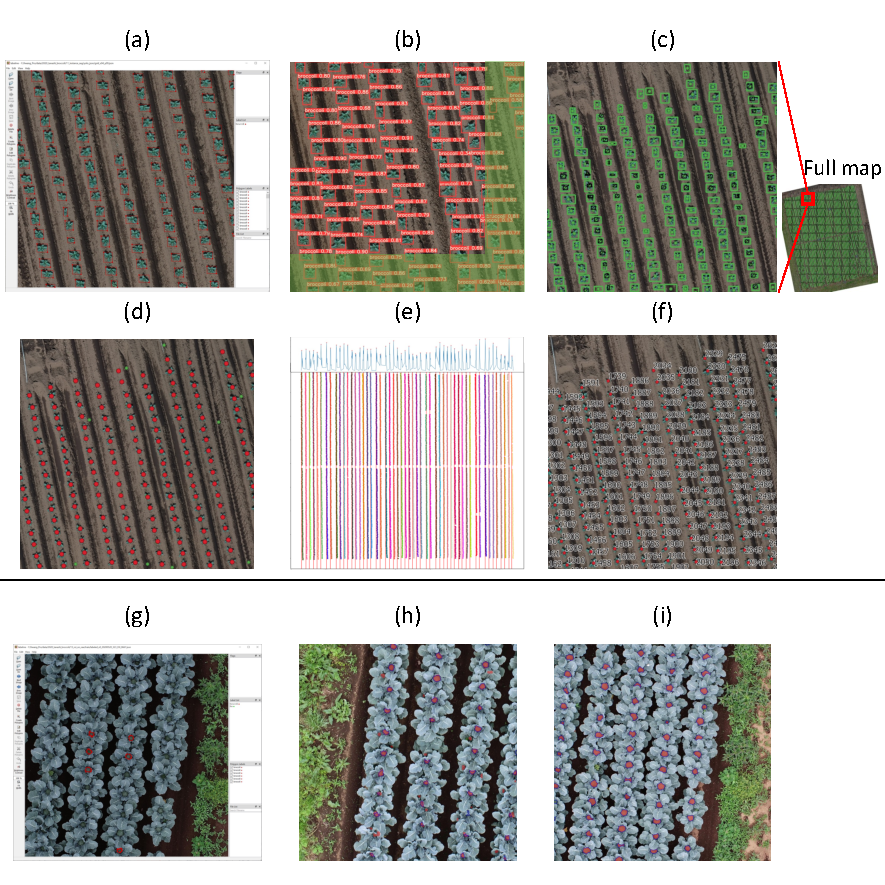
\includegraphics{figures/bro/Fig.S1_deep_learning_demo.pdf}
    }
  \end{center}
  \caption[Examples of 2020 broccoli seedling position detection and head segmentation by interactive annotation]{
    Examples of 2020 broccoli seedling position detection (a-f) and head segmentation by interactive annotation (g-i). 
    (a) One annotated training data by LabelMe. 
    (b) YOLO v5 detected results; the green part is the buffer zone to avoid the broken broccoli at the edge. 
    (c) Duplicate detection in buffer zone removed by the non-maximum suppression (NMS) algorithm. Black shows removed duplicate detection, green shows those that were retained, and green dots are the center points as the broccoli position. 
    (d) Red dots show the manually adjusted positions by QGIS. 
    (e) Ridge detection by identifying the peak of points distribution. 
    (f) Automatic placing of plant ID along the ridge. 
    (g) Startup training data annotation made by LabelMe; only a few annotations were required. 
    (h) After the first iteration. The red polygons are the segmentation results (as auxiliary annotations) trained by the startup data and the blue polygons are manually adjusted according to the previous results. 
    (i) After the fourth iteration, almost no manual adjustment was required in this case.
  }
  \label{fig:bros1}
\end{figure}

\newpage

\begin{landscape}
  \begin{figure}[htb]
  \begin{center}
    \resizebox{\linewidth}{!}{
      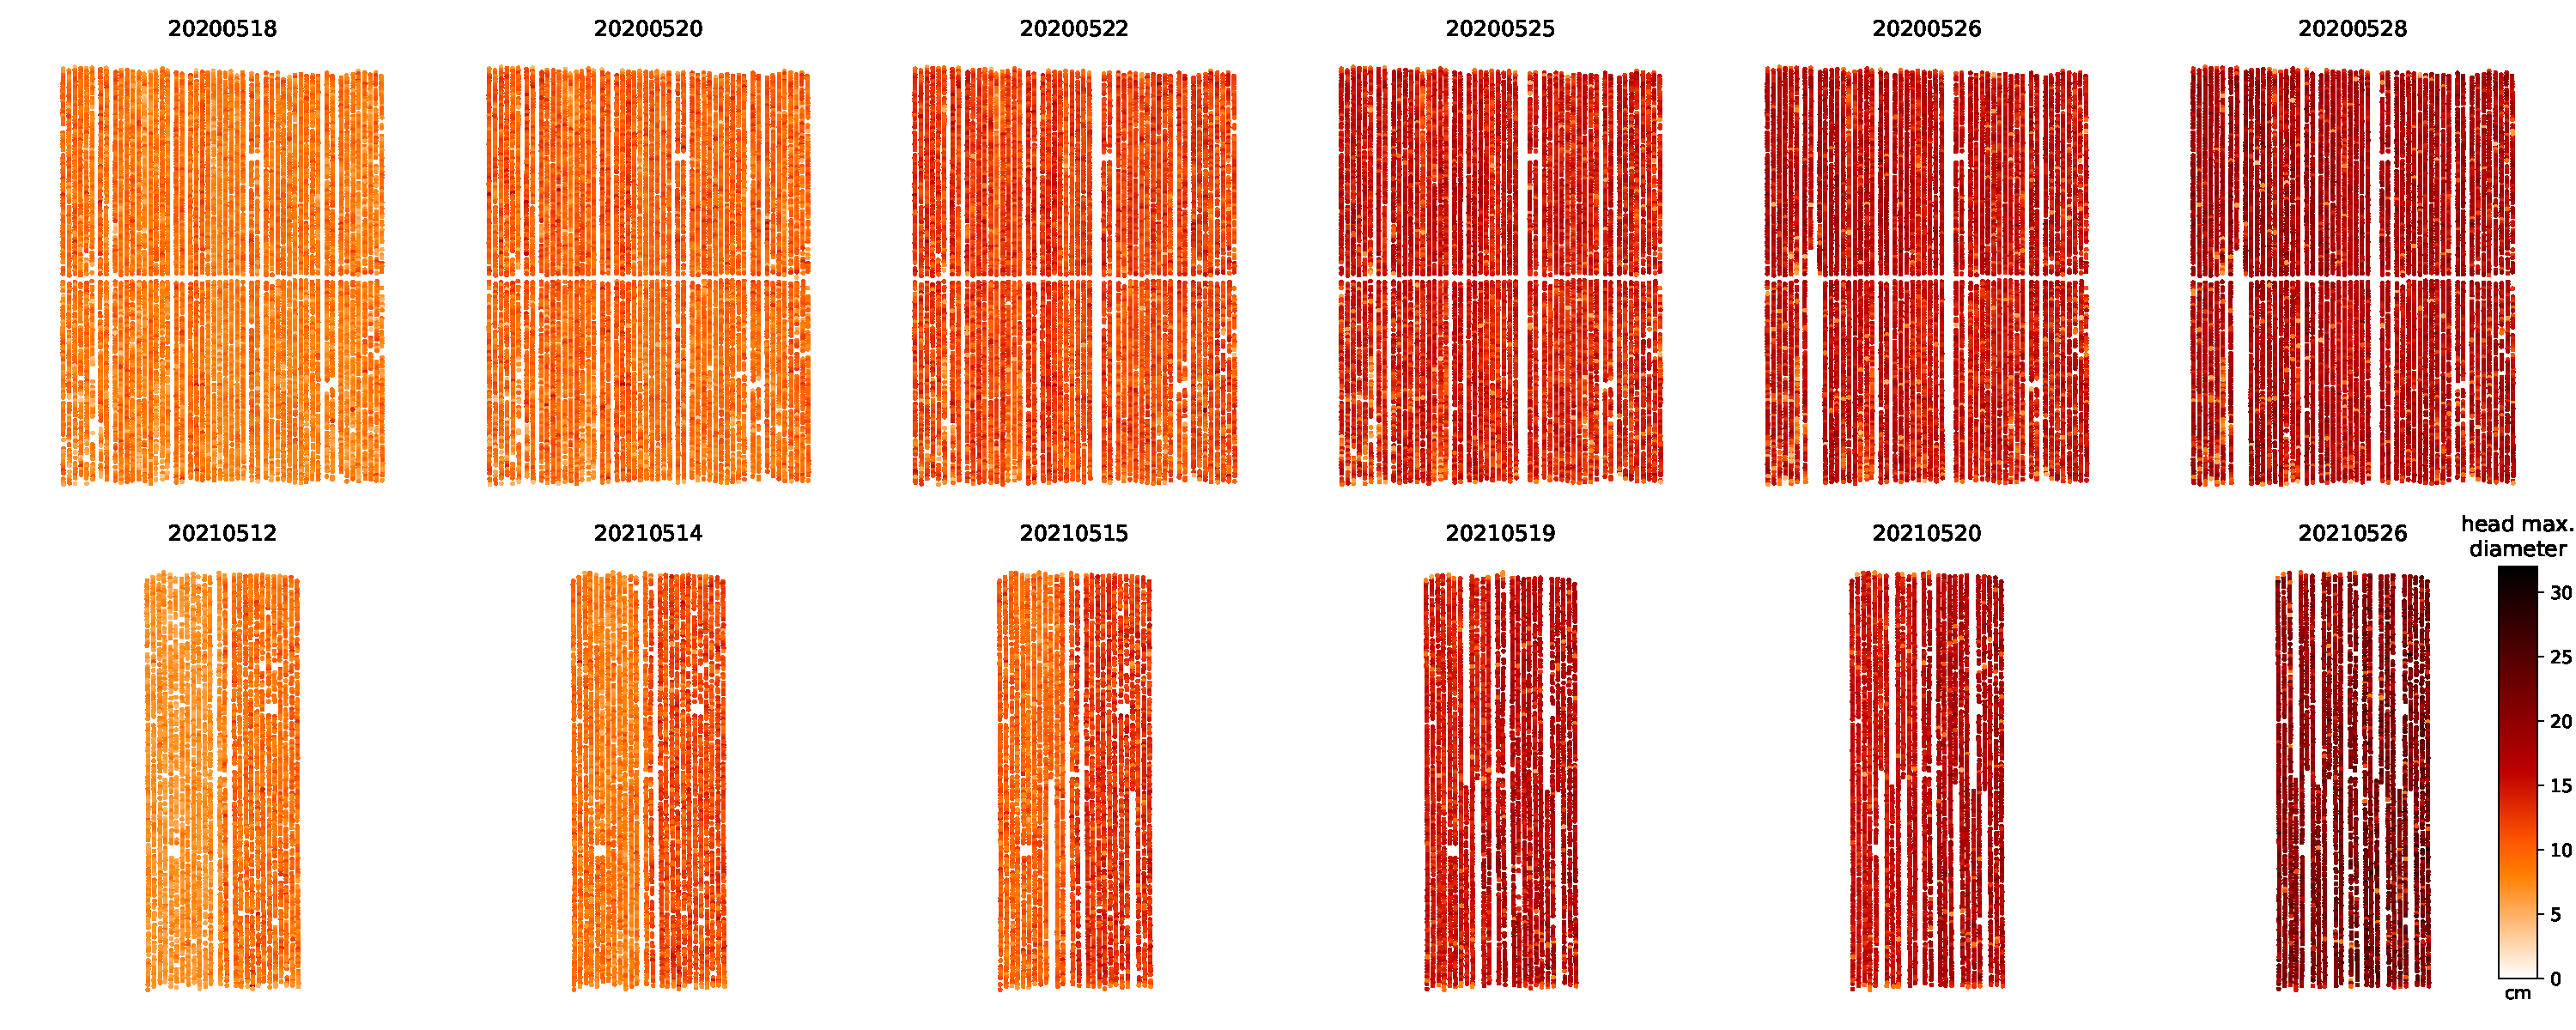
\includegraphics{figures/bro/Fig.S2_plot_heatmap.pdf}
    }
  \end{center}
  \caption[Head size of all broccoli heads based on UAV imagery]{
    Head size of all broccoli heads based on UAV imagery; color represents the maximum head diameter.
  }
  \label{fig:bros2}
\end{figure}
\end{landscape}

% \newpage

% \begin{landscape}
  % \begin{figure}[htb]
  \begin{center}
    \resizebox{0.9\linewidth}{!}{
      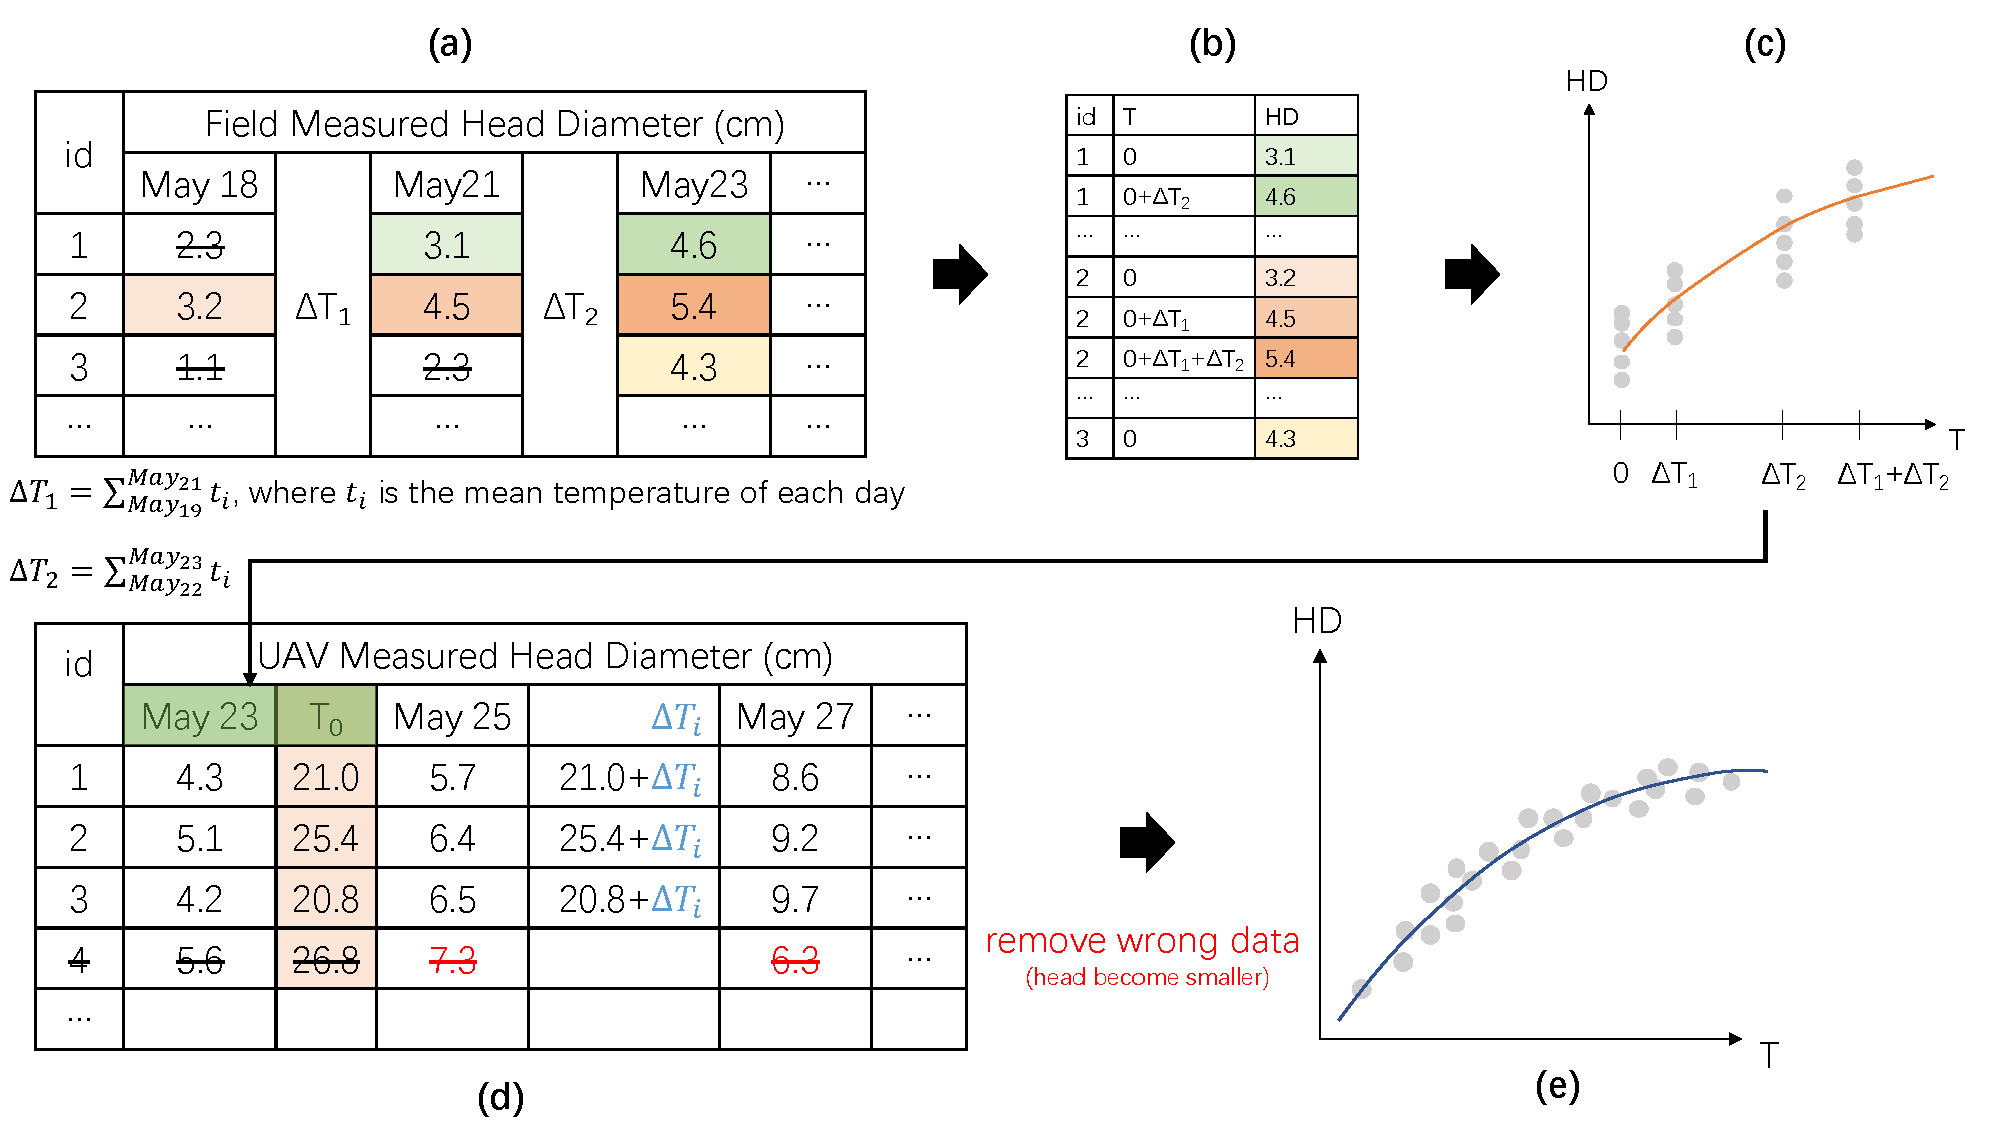
\includegraphics{figures/bro/Fig.S3_yield_workflow.pdf}
    }
  \end{center}
  \caption[Data processing illustration for head size prediction model]{
    Data processing illustration for head size prediction model. All the numbers were just examples, not the actual results. 
    (a) The field-measured measured diameter at on different dates; the light colored was used as the starting date with broccoli head size around of approximately 3-3.5cm. $T$ is the sum of daily average temperature. $\Delta T_i$ is the temperature sum deviation. 
    (b) Reshaping of the previous table to a two-column table for the regression analysis shown in (c). 
    (d) The previous regressed model was used to initialize the $T$ from the head diameter. 
    $T$ on later days was added by the deviation $\Delta T_i$. 
    (e) the previous data was used to regress the prediction model from $T$ to head diameter.
  }
  \label{fig:bros3}
\end{figure}
% \end{landscape}